%% R4Tun — Automation in Construction (cas-dc double-column template)

\documentclass[a4paper,fleqn]{cas-dc}

\usepackage[numbers]{natbib}
\usepackage{booktabs}
\usepackage{multirow}
\usepackage{amsmath}
\usepackage{graphicx}
\usepackage[dvipsnames]{xcolor}
\usepackage{hyperref}

\begin{document}
\let\WriteBookmarks\relax
\def\floatpagepagefraction{1}
\def\textpagefraction{.001}

% ────────────────────────────── Front matter ──────────────────────────────

\shorttitle{R4Tun: LLM-driven adaptive tunnel segmentation}
\shortauthors{X.\ Tao et~al.}

\title[mode=title]{R4Tun: LLM-driven adaptive segmental tunnel lining segmentation in point clouds}

\author[1]{Xinghui Tao}
\credit{Conceptualization, Methodology, Software, Writing -- original draft}

\author[1]{Guangming Wang}
\cormark[1]
\ead{gw462@cam.ac.uk}
\credit{Supervision, Writing -- review \& editing}

\author[2]{Jelena Nini\'{c}}
\credit{Supervision, Writing -- review \& editing}

\author[1]{Brian Sheil}
\credit{Supervision, Funding acquisition, Project administration}

\cortext[cor1]{Corresponding author}

\affiliation[1]{organization={Construction Engineering, University of Cambridge},
    addressline={Trumpington Street},
    city={Cambridge},
    postcode={CB2 1PZ},
    country={United Kingdom}}

\affiliation[2]{organization={Department of Engineering, Durham University},
    addressline={Stockton Road},
    city={Durham},
    postcode={DH1 3LE},
    country={United Kingdom}}

% ─── Abstract ─────────────────────────────────────────────────────────────

\begin{abstract}
Automated inspection of segmental tunnel linings requires adaptive segmentation from 3D point clouds, yet expert-tuned pipelines often degrade when tunnel conditions vary. This limits robust deployment of automated inspection across tunnel networks. This paper presents R4Tun, a large language model (LLM)-driven adaptation framework that augments an expert-designed pipeline (SAM4Tun) with bounded, context-aware parameter tuning using structured context from memory (m), state (s), and knowledge (k). Evaluated on 30 selected Seg2Tunnel subsets spanning 13 regular and 17 complex tunnels across three LLMs, the full design improved mean mIoU by 108.7--118.7\% overall (from 0.150 to 0.313--0.328), by 70.1--83.8\% for regular tunnels (from 0.291 to 0.495--0.535), and by 302.4--321.4\% for complex tunnels (from 0.042 to 0.169--0.177), with state contributing the largest incremental gain (paired Cohen's $d = 1.32$--$1.61$, $p < 0.0001$). Cross-model analysis of 1,350 adapted parameter runs showed convergence on the same critical parameters. These results show that a structured LLM-based system can make tunnel segmentation more adaptive in practice and reduce reliance on repeated expert retuning.
\end{abstract}

% ─── Highlights ───────────────────────────────────────────────────────────

\begin{highlights}

\item Expert-tuned tunnel segmentation degrades when tunnel conditions depart from the reference setting.
\item R4Tun augments an expert-designed pipeline through LLM-driven stage adaptive agents using structured context: memory, state, and knowledge.
\item The framework was validated on 30 tunnel subsets across three LLMs (Opus-4.6, GPT-5.4, Gemini-3), including 17 complex tunnels.
\item Mean mIoU improved by more than 100\% overall with bootstrap 95\% CIs for all three LLMs; per-class IoU improved broadly across all structural classes.
\item Analysis of 270 adapted parameter runs (30 tunnels × 3 LLMs × 3 context settings) showed consistent parameter convergence across LLMs, with state as the main driver of improvement.

\end{highlights}

% ─── Keywords ─────────────────────────────────────────────────────────────

\begin{keywords}
Segmental tunnel lining \sep Point cloud segmentation \sep Tunnel inspection \sep Large language models \sep Parameter adaptation \sep Multi-agent systems
\end{keywords}

\maketitle

\smallskip
% ─────────────────────────────────────────────────────────────────────────

% ══════════════════════════════════════════════════════════════════════════
\section{Introduction}\label{sec:intro}
% ══════════════════════════════════════════════════════════════════════════


Automated inspection of segmental tunnel linings is increasingly required to support structural health assessment and long-term operational safety, given the scale, frequency, and access constraints of modern tunnel networks~\cite{attard2018}. In practice, engineers must work on projects where tunnel geometry, lining conditions, and data acquisition conditions vary substantially ~\cite{weidner2024generalized}. Furthermore, although modern laser-scanning technologies enable high-fidelity tunnel capture, the resulting measurements typically contain mixed structural elements, occlusions, and noise, making direct extraction of lining components challenging ~\cite{huang2021bim,sjolander2023towards}. Consequently, the segmentation methods must be sufficiently adaptive to handle this complexity and variability ~\cite{montero2015, strauss2020sensing, camuffo2022recent}. 

\begin{figure*}[t]
\centering
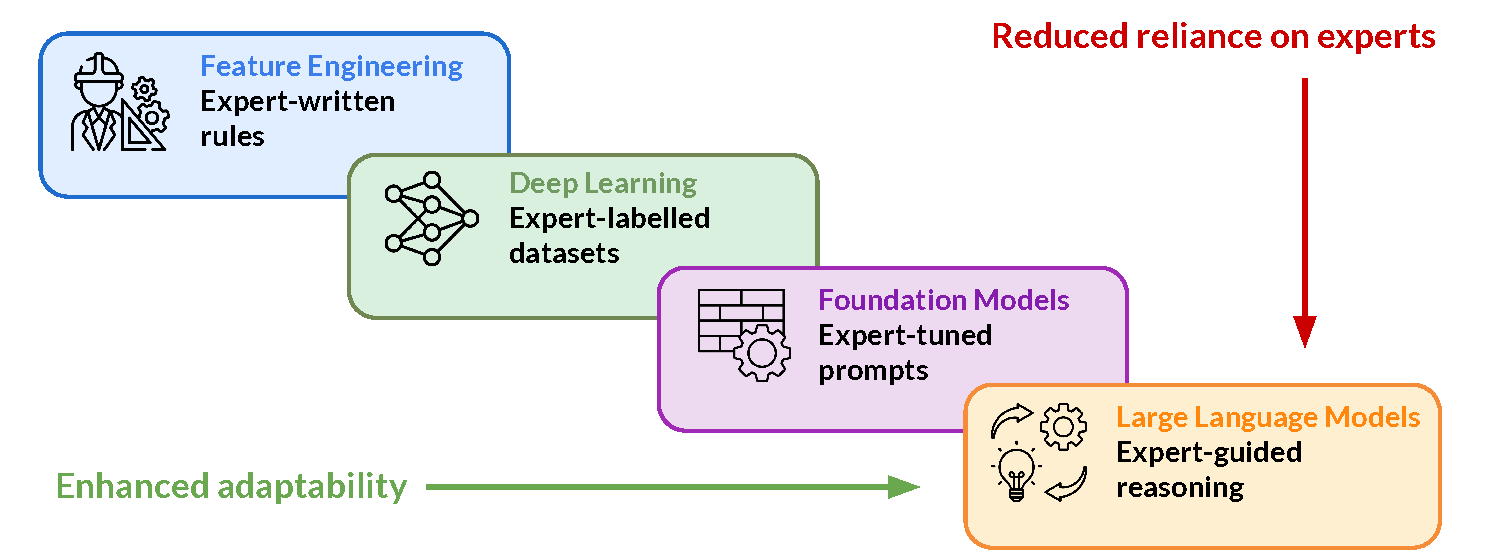
\includegraphics[width=\textwidth]{figs/ai_paradigms.pdf}
\caption{Automated segmentation approaches toward enhanced adaptability. R4Tun extends these approaches by integrating expert–guided reasoning.}
\label{fig:paradigms}
\end{figure*}

Three main approaches exist for tunnel point-cloud segmentation (Fig.~\ref{fig:paradigms}) (Section~\ref{sec:related}). Feature-engineering rules are interpretable but brittle under changed conditions~\citep{weidner2024generalized}. Supervised deep-learning models generalise through data but require large labelled datasets, periodic retraining, and lack interpretability~\citep{cha2024deep, su2024review}. Foundation-model pipelines bypass annotation by leveraging models pre-trained on large datasets~\citep{bommasani2021foundation, kirillov2023sam}, but remain sensitive to expert-tuned processing parameters. None of these approaches simultaneously provides adaptability to new conditions and interpretability of the adaptation process. Among foundation-model pipelines, SAM4Tun~\citep{ye2025sam4tun} combines point-cloud preprocessing with SAM-based prompting~\citep{kirillov2023sam} and has demonstrated strong performance under expert tuning. However, it remains highly sensitive to its approximately 80 preprocessing and prompting parameters: deviations in tunnel geometry or scanning conditions from those assumed during tuning can result in sharp performance degradation, causing repeated expert retuning, increased quality assurance effort, and reduced confidence in operational automation.



Recent advances in natural language processing (NLP) have enabled an alternative approach. Large language models (LLMs) are increasingly embedded in engineering workflows as general-purpose assistants \citep{bradley2023chemcrow, ghafarollahi2024protagents, qian2024chatdev, hong2024metagpt, chen2024comm, garcia2024manufacturing}. We therefore propose R4Tun, an LLM-driven adaptation system that augments the SAM4Tun pipeline by adjusting stage parameters in response to changing tunnel conditions without expert tuning. The framework provides each LLM agent with structured context comprising memory (reference tunnel characteristics), state (intermediate pipeline outputs), and knowledge (domain-specific tuning guidelines), from which the agent produces bounded parameter updates via chain-of-thought (CoT) reasoning. We evaluate whether this structured context improves segmentation adaptability across regular and complex tunnels, and whether the adaptation behaviour is consistent across independent LLMs.

This paper makes the following contributions:
\begin{enumerate}
\item A framework design in which LLM agents adapt the parameters of SAM4Tun pipeline using structured context without modifying the pipeline’s algorithms.
\item A cumulative ablation methodology that isolates the incremental contribution of each context component (m, s, k) to segmentation performance across 30 tunnels under varying conditions.
\item Cross-LLM validation showing that three independent LLMs (Opus-4.6, GPT-5.4, Gemini-3) produce statistically consistent adaptation patterns, converging on the same critical parameters.
\end{enumerate}

The rest of this paper is organised as follows. Section~\ref{sec:related} reviews related work. Section~\ref{sec:methods} presents materials and methods, including the R4Tun architecture, dataset, experimental design, and evaluation. Section~\ref{sec:results} reports results. Section~\ref{sec:discussion} discusses findings, implications, and limitations. Section~\ref{sec:conclusions} concludes.

% ══════════════════════════════════════════════════════════════════════════
\section{Related work}\label{sec:related}
% ══════════════════════════════════════════════════════════════════════════

\subsection{Feature-engineering vs Deep-learning}

Tunnel point-cloud segmentation has advanced through two major generations of methods, each solving one problem while leaving another open. Feature-engineering approaches encode domain knowledge into deterministic geometric rules: centreline fitting via RANSAC ~\cite{fischler1981ransac}, density-based surface clustering ~\cite{ester1996dbscan}, and multi-scale curvature analysis ~\cite{pauly2002}. Those methods remain widely used in safety-critical inspection because their logic is explicit and auditable ~\cite{weidner2024generalized}. However, each rule embeds assumptions about certain tunnel geometry and point cloud characteristics (diameter, ring spacing, joint pattern, point density), and changing any of these requires manual reconfiguration by a domain expert. Supervised deep-learning methods, such as PointNet++~\cite{qi2017pointnet}, RandLA-Net~\cite{hu2020randla}, Mask3D~\cite{schult2023mask3d}, TD3D~\cite{kolodiazhnyi2024td3d} learn features directly from annotated point clouds and can generalise across similar conditions present in the training set. Yet they require large labelled tunnel datasets that remain scarce~\cite{su2024review}, demand retraining for new tunnel conditions, and provide no mechanism for an engineer to trace or override a segmentation decision~\cite{cha2024deep}.

The tension that persists across both generations is structural: methods that are interpretable are not adaptive, and methods that adapt through data are not interpretable. For inspection operators, this means every deployment to a new tunnel type requires either re-engineering rules, collecting new training data, or accepting degraded performance without a systematic way to diagnose the cause.

\subsection{Foundation-model pipelines}

No foundation model currently exists for direct 3D point-cloud segmentation; available models operate on 2D images. To leverage their capabilities, tunnel pipelines must first project 3D point clouds into 2D representations. Among 2D vision foundation models, those pre-trained on large-scale image datasets offer a third route that bypasses the annotation bottleneck entirely. SAM~\cite{kirillov2023sam} performs class-agnostic segmentation from spatial prompts without task-specific training, and extensions such as SAM2~\cite{ravi2024sam2} for temporal consistency and SEEM~\cite{zou2023segment} for natural-language-guided segmentation are broadening prompt-based segmentation further. These models have been adopted in infrastructure contexts including crack detection~\cite{ravi2024cracksam} and Scan-to-BIM workflows~\cite{wang2024omni}.

For tunnel linings, SAM4Tun~\cite{ye2025sam4tun} combines geometric preprocessing (unfolding, denoising, enhancement and Hough-based detection with prompting), achieving strong segmentation without training data. However, this pipeline depends on approximately 80 parameters across stages that encode assumptions about the reference tunnel's diameter, ring length, point density, and joint patterns. When a new tunnel departs from the reference, these parameters become misspecified and the pipeline degrades silently, without signalling which parameters are failing or why. This sensitivity is not unique to SAM4Tun: any multi-stage pipeline that chains domain-specific preprocessing with a foundation model inherits it. Foundation models have reduced reliance on labelled data and increased the interpretability of parameter choices and prompts, but they have not reduced reliance on expert parameter tuning.

\subsection{LLM reasoning}

Recent LLM advances have introduced explicit reasoning capabilities relevant to the parameter-adaptation problem. CoT reasoning~\cite{wei2023cot} enables step-by-step logical traces. Training techniques, especially reinforcement learning~\cite{deepseek2025analysis, openai2025o3, xiang2025metacot}, produce models capable of decomposing complex problems and self-verifying intermediate steps. Multi-agent architectures coordinate specialized roles through shared context~\cite{hong2024metagpt, qian2024chatdev, chen2024comm}, and context engineering strongly influences reasoning quality through the systematic design of information provided to models~\cite{xu2024retrieval, mei2025survey}.

In tunnelling segmentation, however, no work has applied LLM-based reasoning to the specific problem that foundation-model pipelines face: how to retune a parameter-sensitive system for new conditions while preserving the engineer’s ability to inspect and override every decision. This gap motivates the present study.


% ══════════════════════════════════════════════════════════════════════════
\section{Methodology}\label{sec:methods}
% ══════════════════════════════════════════════════════════════════════════

\subsection{Task definition}\label{sec:problem-def}

The task is semantic segmentation of segmental tunnel linings from terrestrial laser scanning (TLS) point clouds. Given a raw point cloud of a tunnel section, the goal is to assign each point a structural label: background, key block~(K), base blocks (B1,~B2), and adjacent blocks (A1--A3), with an additional A4 class for 7-segment complex tunnels. The unit of analysis is a tunnel subset spanning multiple rings selected from the Seg2Tunnel benchmark. 

The practical problem is that the fixed configuration of the open-source SAM4Tun achieves a mean mIoU of 0.367 on regular (alternating) tunnels, for which it is tuned, but only 0.042 on complex tunnels whose geometry departs from the tuning reference. This degradation is silent: the pipeline does not signal which parameters are misspecified or why performance has declined.

\subsection{Baseline: SAM4Tun}\label{sec:baseline}

R4Tun augments rather than replaces SAM4Tun~\cite{ye2025sam4tun}, so the baseline pipeline is described first. SAM4Tun processes tunnel point clouds through five sequential stages:

\textbf{Stage~1-Unfolding} (Fig.~\ref{fig:stage-u}) establishes a cylindrical coordinate system for the tunnel. It slices the point cloud at regular longitudinal intervals, fits an ellipse to each cross-section via RANSAC~\cite{fischler1981ransac}, and selects the model with the highest inlier support. The per-slice ellipse centres are interpolated into a smooth centreline that defines the cylindrical frame~$(r, \theta, h)$. The 3D tunnel surface is then projected into a 2D panoramic image in which each pixel encodes the radial distance to the centreline, producing a stable depth representation for downstream filtering and segmentation.

\begin{figure*}[t]
\centering
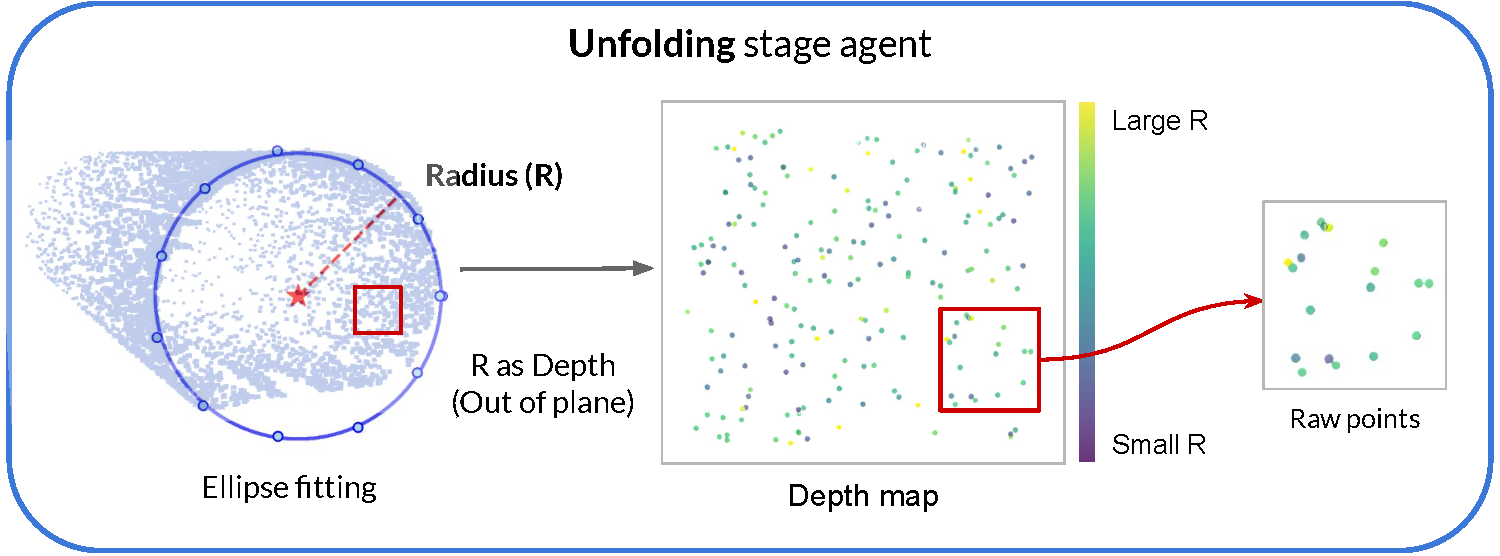
\includegraphics[width=0.8\textwidth]{figs/stage_u.pdf}
\caption{Stage 1-Unfolding. Left: fitted tunnel cross-section used to determine the reference centre and radius for cylindrical unfolding. Centre: 2D panoramic depth map derived from the 3D point cloud. Right: zoomed region of the unfolded map showing radial-distance encoding.}
\label{fig:stage-u}
\end{figure*}

\textbf{Stage~2-Denoising} (Fig.~\ref{fig:stage-d}) removes non-structural artefacts (rails, cables, and scattered points) that would otherwise interfere with segmentation. The algorithm applies grid-based radial-density filtering inspired by the DBSCAN clustering principle~\cite{ester1996dbscan}, grouping points by local density in cylindrical coordinates. Dense, connected regions are retained as tunnel surfaces while isolated points are rejected as noise. A pair of radial masks~($R_\mathrm{low}$, $R_\mathrm{high}$) constrains filtering to the expected tunnel radius, preserving joint boundaries and ring edges while discarding outliers beyond the lining surface. The result is a clean, continuous surface representation suitable for curvature analysis and interpolation in the next stage. 

\begin{figure*}[t]
\centering
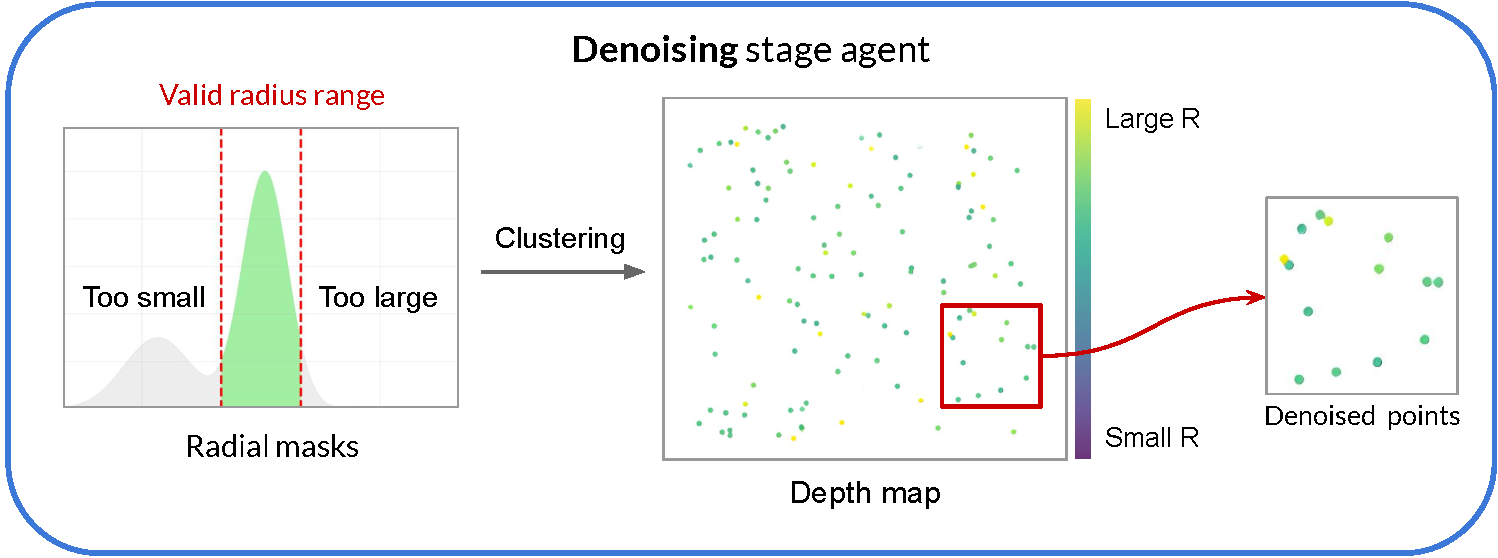
\includegraphics[width=0.8\textwidth]{figs/stage_d.pdf}
\caption{Stage 2-Denoising. Left: radial-distance distribution used to filter points outside the expected tunnel lining surface. Centre: unfolded 2D depth map after filtering, showing the cleaned point distribution. Right: zoomed region of the denoised map.}
\label{fig:stage-d}
\end{figure*}

\textbf{Stage~3-Enhancing} (Fig.~\ref{fig:stage-e}) improves geometric continuity and surface completeness before projection into the 2D depth map. Local curvature is estimated on neighbourhood points to guide point insertion: new points are placed between neighbours whose curvature difference is small (smooth panel regions), while high-curvature areas (joint boundaries and ring edges) are preserved intact. A three-stage progressive upsampling scheme inserts additional points at progressively finer resolutions to maintain surface continuity without blurring structural boundaries. Pixel-level interpolation then refines outlier points at joint locations. The enhanced surface is projected into a panoramic depth map that balances smooth panel regions with sharply defined joint boundaries. 

\begin{figure*}[t]
\centering
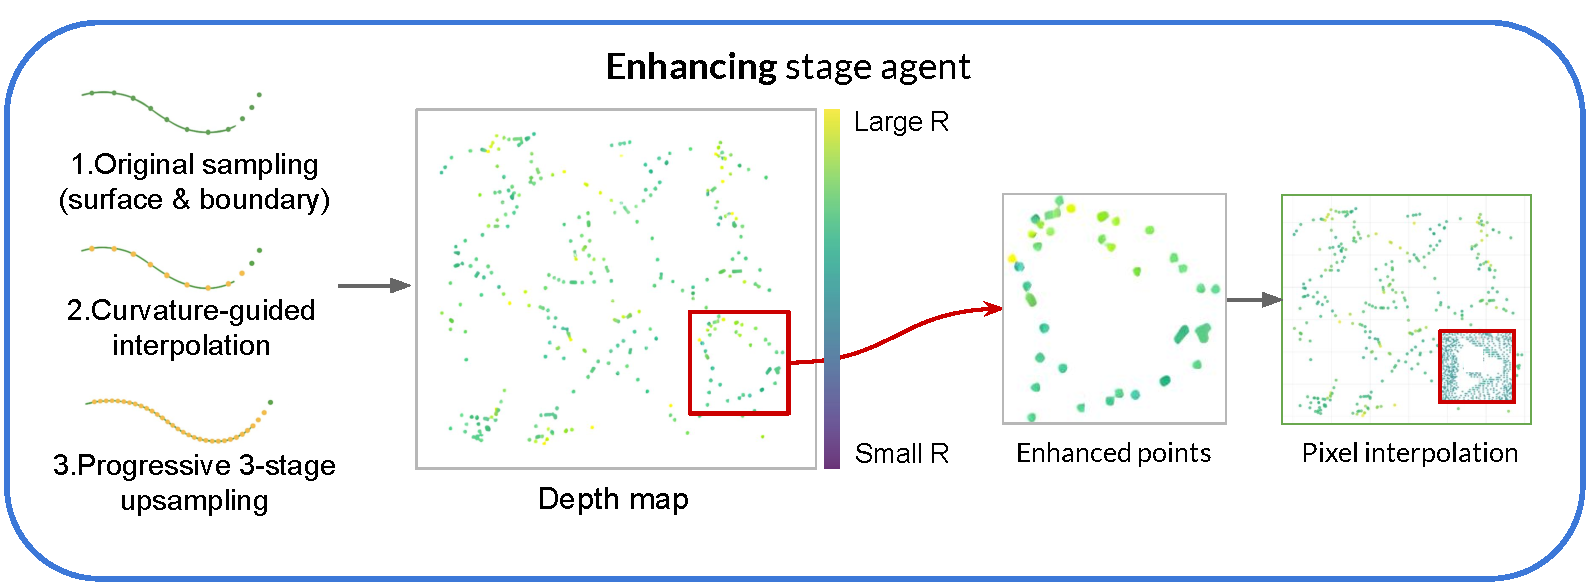
\includegraphics[width=0.8\textwidth]{figs/stage_e.pdf}
\caption{Stage 3-Enhancing. Left: curvature-guided surface and boundary interpolation along the tunnel lining, showing original sampling, curvature-guided insertion, and progressive three-stage upsampling. Centre: unfolded 2D depth map after enhancement, where inserted points improve geometric continuity; the red box highlights a local region of interest. Right: zoomed views of the highlighted region, showing added points and pixel-level interpolation.}
\label{fig:stage-e}
\end{figure*}

\textbf{Stage~4-Segmenting} (Fig.~\ref{fig:stage-p}) combines boundary detection and SAM segmentation into a single workflow. First, a Hough-transform-based detector~\cite{duan2023high} extracts linear features from the enhanced depth map that correspond to ring joint boundaries. Detected lines are filtered by orientation (oblique, horizontal, vertical) with separate Hough thresholds and merged when closer than a distance tolerance. The confirmed boundaries are then used to construct template-based prompts for key, base, and adjacent segments, which are passed to SAM~\cite{kirillov2023sam}. SAM produces 2D segment masks on the panoramic image, which are reprojected into 3D point labels via the stored pixel-to-point mapping from Stage~1. 

\begin{figure*}[t]
\centering
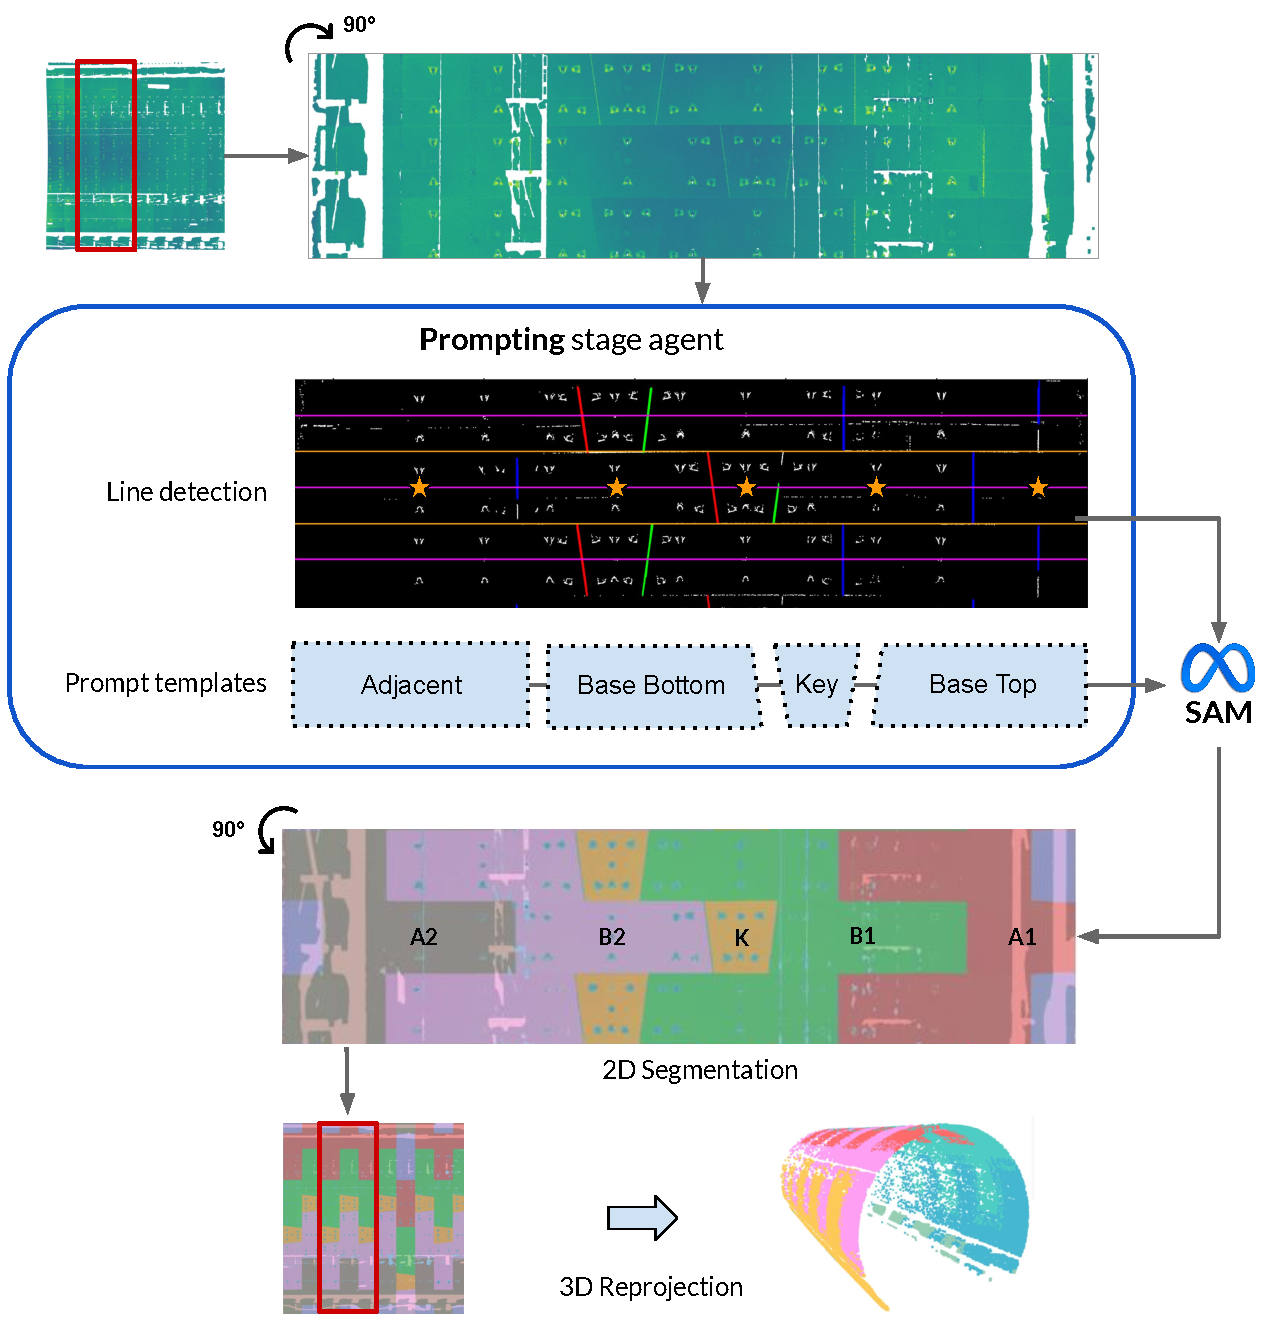
\includegraphics[width=0.8\textwidth]{figs/stage_p.pdf}
\caption{Stage~4-Prompting \,\& Stage~5---Segmenting: Hough-transform line detection to identify ring boundaries, constructs template-based prompts, and feeds them to SAM~\cite{kirillov2023sam}, which produces 2D segment masks that are reprojected into 3D. (Note: rotation is shown for visualisation purposes only.)}
\label{fig:stage-p}
\end{figure*}

The pipeline contains approximately 80 tuneable processing parameters. All parameters were expert-tuned on a reference tunnel (diameter 5.60\,m, density 2{,}466\,pts/m$^3$, mIoU\,=\,0.531); full parameter tables are provided in Appendix~\ref{app:params}. In this study, the five stage algorithms remain fixed across all conditions; only the parameter values change. The \texttt{sam4tun} baseline applies this single expert-tuned configuration uniformly to all 30 tunnels without per-tunnel adaptation, serving as the rule-only reference against which LLM-driven adaptation is measured.

\subsection{R4Tun}\label{sec:method}

R4Tun augments the fixed SAM4Tun pipeline with an LLM-driven adaptation layer that adjusts parameters per tunnel without modifying the underlying algorithms (Fig.~\ref{fig:architecture}). Given a new tunnel point cloud, a characteriser first extracts raw geometric properties (diameter, density, coordinate ranges; full field list in Appendix~\ref{app:chars}). The first four stages (unfolding, denoising, enhancing, prompting) each have a dedicated LLM agent that adapts their parameters; the final segmentation stage passes the adapted prompts directly to SAM without further LLM intervention. 

For each agent-driven stage, (i)~the orchestrator assembles a structured prompt from the current context level (m, s, k) (Section~\ref{sec:context-comp}); (ii)~the LLM reasons over this prompt via CoT and returns an adapted parameter JSON (Section~\ref{sec:cot}); (iii)~the stage runs with the adapted parameters; and (iv)~a characteriser plugin extracts structured statistics from the output, updating the state available to subsequent stages. Each stage's parameters are inferred independently from the expert-tuned reference configurations. The stage scripts and evaluation code are identical across all ablation conditions; only the parameter JSONs change. A worked example of this process is provided in Appendix~\ref{app:cot}. After the final segmentation, per-point labels are evaluated against ground truth using mean Intersection over Union (mIoU) as the primary metric.

\begin{figure*}[t]
\centering
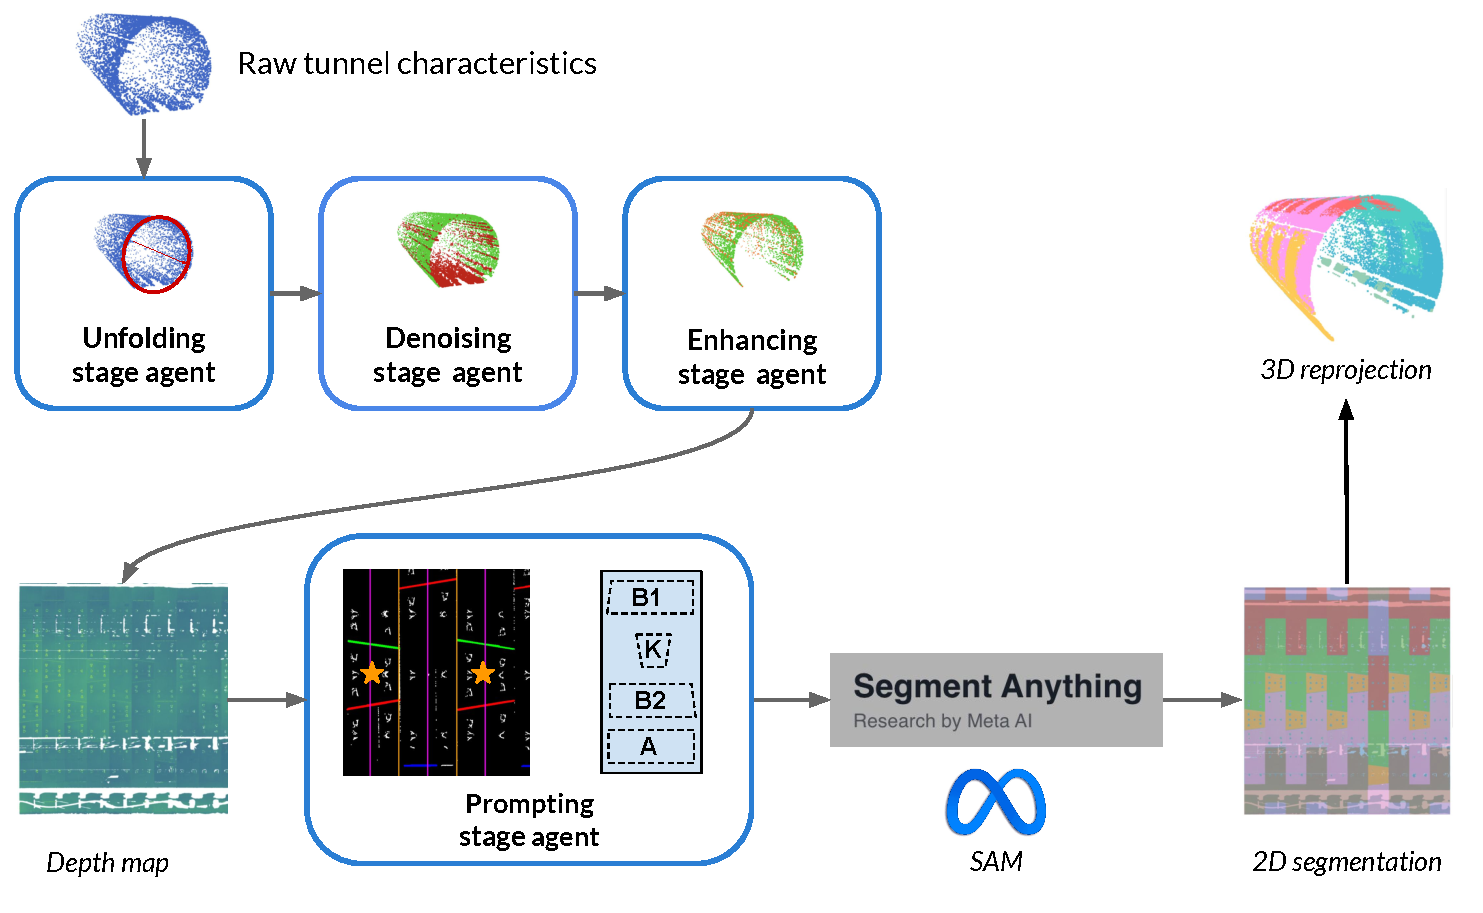
\includegraphics[width=0.8\textwidth]{figs/r4tun_pipeline.pdf}
\caption{The R4Tun multi-agent architecture for tunnel segmentation. Four stage agents (unfolding, denoising, enhancement, and prompting) adapt their parameters through LLM reasoning to generate segmentation.}
\label{fig:architecture}
\end{figure*}

\begin{figure*}[t]
\centering
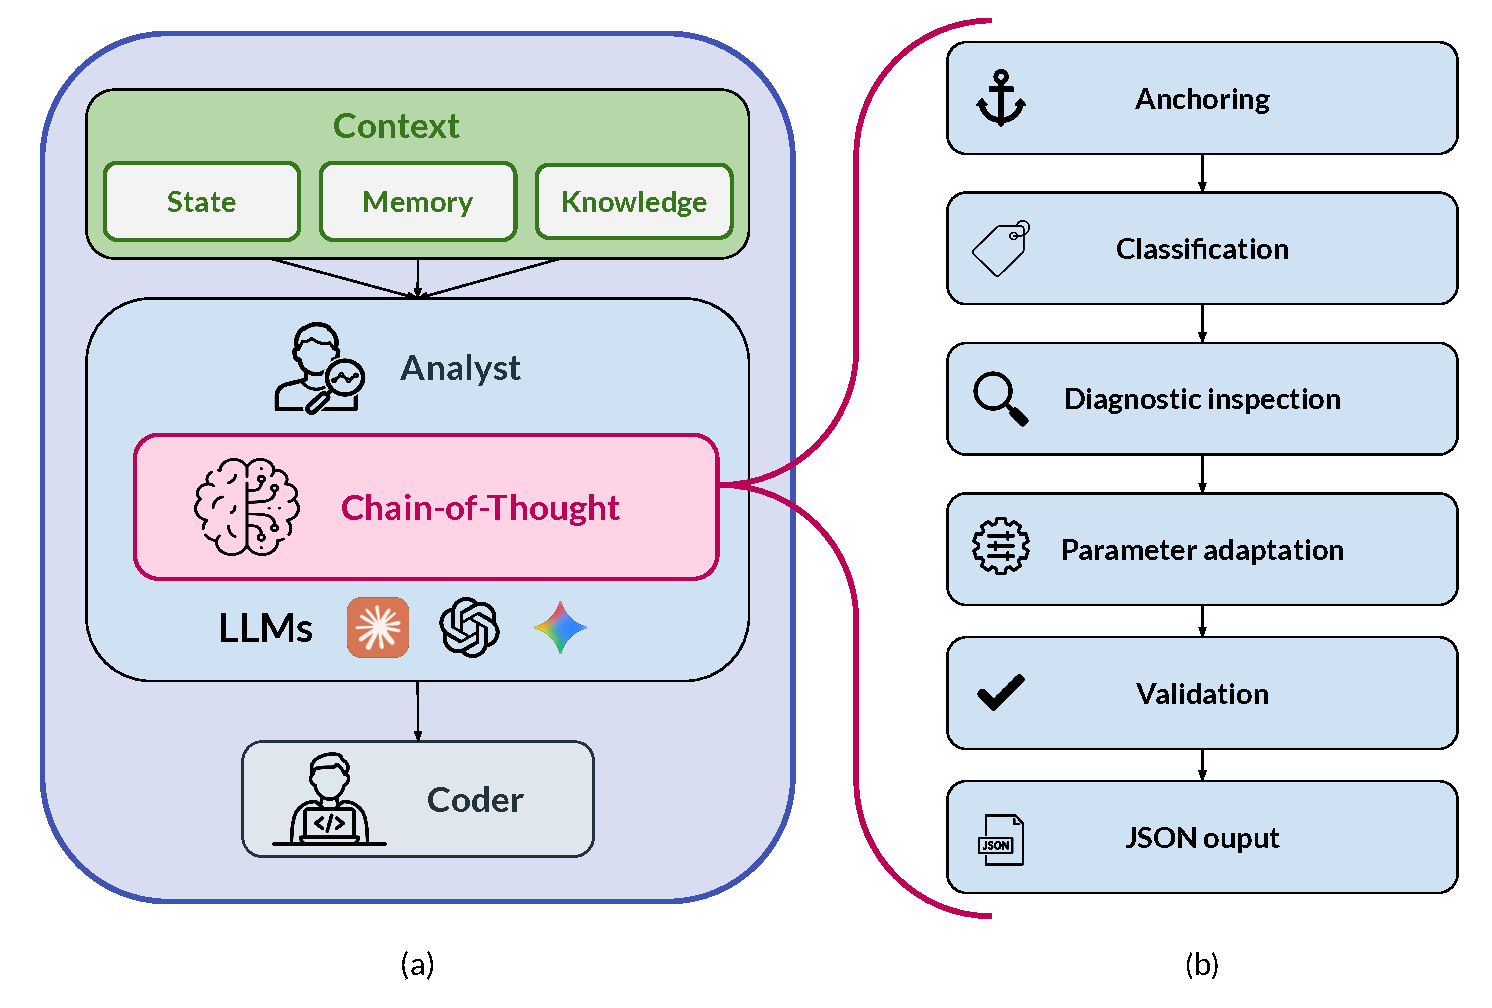
\includegraphics[width=0.8\textwidth]{figs/agent_design.pdf}
\caption{The left column (a) shows R4Tun stage agent architecture. Each agent maintains an evolving context (m, s, k) that informs a LLM analyst component performing CoT reasoning; The right column (b) shows the five CoT phases: (1) Referencing, (2) Diagnostic inspection, (3) Parameter adaptation, (4) Validation, and (5) JSON output.}
\label{fig:agent-design}
\end{figure*}

\subsubsection{Agent design}\label{sec:agent-design}

Each of the four stage agents is a self-contained unit comprising three components: a \emph{context} assembled from m, s and k (Section~\ref{sec:context-comp}) (Fig.~\ref{fig:agent-design}a), and a \emph{LLM analyst} function that constructs the full LLM prompt and parses the returned JSON. Within this prompt, the analyst embeds a structured five-step CoT protocol (Section~\ref{sec:cot}) (Fig.~\ref{fig:agent-design}b) that guides the LLM through anchoring, classification, diagnosis, adaptation, and validation. The LLM then outputs a single schema-conformant parameter JSON, which the corresponding pipeline stage executes unchanged. Because every parameter change is linked to an explicit reasoning trace, engineers can inspect, interpret, and override any adaptation decision.

\subsubsection{Context design}\label{sec:context-comp}

Each stage agent receives structured context comprising three components: memory, state and knowledge (Fig.~\ref{fig:agent-design}a).

\textbf{Memory} stores the reference tunnel's characteristics (a JSON file containing geometry, point density, coordinate ranges, nearest-neighbour distances) alongside the expert-tuned reference parameters. The agent compares the current tunnel's characteristics against this reference to quantify deviation and adjust its parameters. Memory is static: it does not change between stages.

\textbf{State} captures cumulative geometric and statistical properties after each pipeline stage executes. After each stage, a characteriser plugin extracts a structured JSON summary. These cumulative summaries are injected into subsequent agents' prompts. State is dynamic: it grows as stages execute. Critically, state operates through the LLM reasoning process: the raw numeric summaries must be interpreted in the context of parameter semantics and tunnel conditions before they can inform parameter updates.

\textbf{Knowledge} supplies domain-specific guidance in human-readable markdown documents. Each stage has its own knowledge document covering: tunnel-type taxonomy; parameter semantics and empirically validated ranges; and diagnostic rules linking characteristics to parameter adjustments. Knowledge is authored once and shared across all tunnels.

\subsubsection{CoT design}\label{sec:cot}

CoT reasoning provides the analytical structure for each agent's decision-making (Fig.~\ref{fig:agent-design}b). Each stage agent follows a five-step protocol: (i)~\emph{anchoring} compares the current tunnel's characteristics against the stored reference to quantify deviation; (ii)~\emph{diagnostic inspection} attributes the deviation to a plausible cause and identifies which stage parameters are implicated; (iii)~\emph{parameter adaptation} proposes bounded updates within empirically predefined ranges, grounded in the diagnostic evidence and domain knowledge; and (iv)~\emph{validation} performs a lightweight consistency check to confirm that the proposed values satisfy logical constraints. (v) The agent then packages the selected parameters and their reasoning trace into a single schema-conformant JSON object, which is executed by the underlying pipeline-stage function. A worked example of the full five-step trace is provided in Appendix~\ref{app:cot}.

\subsection{Experimental setup}\label{sec:exp-setup}

\subsubsection{Dataset}\label{sec:dataset}

We selected 30 tunnel subsets from the Seg2Tunnel benchmark(Table~\ref{tab:dataset}). These subsets systematically vary in diameter, ring length, segment count, key-block layout, and point-density distribution, yielding a sufficiently diverse evaluation design. 

Staggered and continuous tunnels are grouped as ``regular'' ($n = 13$): they share the 5.5\,m nominal diameter, 1.2\,m ring spacing, six segments per ring, and, most importantly, regular patterns of key-block positions similar to the reference. Complex tunnels ($n = 17$) depart from that reference in multiple coupled ways: inner diameter increases by 36\% (7.5\,m), ring length by 50\% (1.8\,m), and each ring adds a seventh segment with a complex interleaved key-block arrangement. In addition, Off-axis scanning yields non-uniform sampling, partial circumferential coverage, and angle-dependent range and incidence. Together, these differences change both the geometry seen in the point cloud and the semantic targets the pipeline must recover, so a fixed parameter set cannot be assumed to transfer from the regular reference; these conditions constitute the primary stress test for whether R4Tun can adapt the same algorithmic pipeline to off-design tunnel conditions. Ground-truth labels are per-point structural class annotations provided by the Seg2Tunnel benchmark; they are used for evaluation only and are not provided to the LLM or pipeline during adaptation.

\begin{table*}[t]
\caption{Dataset properties.}\label{tab:dataset}
\begin{tabular*}{\textwidth}{@{\extracolsep{\fill}} l l l l @{}}
\toprule
 & \multicolumn{2}{c}{Regular (T1, T2, T3)} & Complex (T4, T5) \\
\cmidrule(lr){2-3}\cmidrule(l){4-4}
Property & Staggered (T1, T2) & Continuous (T3) & \\
\midrule
Inner diameter & 5.5\,m & 5.5\,m & 7.5\,m \\
Ring length & 1.2\,m & 1.2\,m & 1.8\,m \\
Segments/ring & 6 & 6 & 7 \\
Joint type & Staggered & Continuous & Complex interleaved \\
Key-block position & \parbox[t]{0.30\textwidth}{\raggedright A ring-to-ring repeating pattern} & \parbox[t]{0.20\textwidth}{\raggedright A fixed ring-wise order} & \parbox[t]{0.20\textwidth}{\raggedright No repeating pattern} \\
Scanning & Single-station & Multi-station & Single-station, offset \\
Eval.\ schema & 6-class & 6-class & 7-class \\
Count & 10 subsets & 3 subsets & 17 subsets \\
\bottomrule
\end{tabular*}
\end{table*}

\subsubsection{Experimental design}\label{sec:comparators}

The experiment follows a cumulative ablation design with four conditions, each adding one context component (Table~\ref{tab:ablation}). This design isolates the incremental contribution of each component while maintaining a consistent comparison framework. Level~0 (\texttt{SAM4Tun}) is the fixed expert-tuned baseline with no LLM involvement. Levels~1--3 progressively provide the LLM with richer context, enabling the cumulative ablation to attribute improvements to specific components. 

\begin{table}[ht]
\caption{Ablation conditions.}\label{tab:ablation}
\begin{tabular*}{\tblwidth}{@{} c l l >{\raggedright\arraybackslash}p{2.75cm} @{\hspace{0.7em}}@{}}
\toprule
Level & Code & Condition & What the LLM sees \\
\midrule
0 & SAM4Tun & Baseline & Fixed default parameters \\
1 & m & Memory & Reference characteristics + parameters \\
2 & m+s & Memory+State & + intermediate pipeline outputs \\
3 & m+s+k & \begin{tabular}[t]{@{}l@{}}Memory + State + \\ Knowledge\end{tabular} & + domain knowledge \\
\bottomrule
\end{tabular*}
\end{table}



To assess whether adaptation behaviour depends on a specific LLM, each condition was run with three independent LLMs (Opus-4.6, GPT-5.4, and Gemini-3-Flash) under identical prompts. Fairness across conditions is maintained by keeping the pipeline code, evaluation scripts, and prompt structure identical; only the context content varies. Each of the three ablation conditions was run once per LLM for all 30 tunnels, yielding $3 \times 3 \times 30 = 270$ pipeline executions plus 30 baseline runs with fixed parameters. All three LLMs were accessed via their respective commercial APIs (Table~\ref{tab:llm-config}). No model-specific prompt tuning was performed.

\begin{table}[ht]
\caption{LLM configuration.}\label{tab:llm-config}
\begin{tabular*}{\tblwidth}{@{} l l @{}}
\toprule
Setting & Value \\
\midrule
Models & Opus-4.6, GPT-5.4, Gemini-3-Flash \\
Max tokens & 16{,}384 \\
Temperature & Default (API default, not overridden) \\
Timeout & 300\,s per call \\
Prompt format & Markdown with JSON code \\
Failure handling & JSON extraction fail $\rightarrow$ log \& error \\
\bottomrule
\end{tabular*}
\end{table}



Pipeline execution used a single NVIDIA RTX~5060 GPU. Adapted parameter files and CoT reasoning traces were logged for all runs, enabling post-hoc sensitivity analysis (Section~\ref{sec:sensitivity-method}).

\subsubsection{Evaluation metrics}\label{sec:metrics}

Segmentation quality is measured by mean Intersection-over-Union (mIoU):
\begin{equation}
\text{IoU}_c = \frac{\text{TP}_c}{\text{TP}_c + \text{FP}_c + \text{FN}_c}, \qquad
\text{mIoU} = \frac{1}{C} \sum_{c=1}^{C} \text{IoU}_c,
\end{equation}
where $C = 6$ (regular) or $C = 7$ (complex). Overall accuracy (OA) and macro~F1 are also computed; mIoU is the primary metric. Per-class IoU is reported to assess whether improvements are broad or concentrated in specific structural classes.

For each condition and LLM, paired differences $\Delta_i = \text{mIoU}_{\text{condition},i} - \text{mIoU}_{\text{baseline},i}$ were computed for each tunnel~$i$, with $n = 13$ (regular), $n = 17$ (complex), or $n = 30$ (all tunnels). Three complementary statistics support interpretation of the reported improvements: (i)~the \emph{p}-value (paired $t$-test, two-sided, $\alpha = 0.05$) indicates whether an observed difference likely reflects a real performance change rather than random variation; a small value (e.g.\ $p < 0.0001$) means the gain is very unlikely to have arisen by chance; (ii)~the 95\,\% confidence interval gives the plausible range of the true mean improvement; if the entire interval lies above zero the data support a genuine positive gain, and when CIs for different LLMs overlap their mean gains are not clearly separated by model choice alone; (iii)~the effect size (paired Cohen's $d = \bar{\Delta}/s_\Delta$) quantifies practical magnitude, where $|d| \approx 0.2$, $0.5$, and $0.8$ are conventionally small, medium, and large, and values well above~$1$ indicate that nearly every tunnel improved. Results combining very small $p$-values, positive 95\,\% CIs, and large effect sizes provide the strongest evidence that the observed gains are both statistically reliable and practically meaningful.


\subsubsection{Sensitivity analysis}\label{sec:sensitivity-method}

To assess the robustness of adapted parameters, we analysed 1{,}350 adapted parameter files ($30~\text{tunnels} \times 3~\text{LLMs} \times 3~\text{conditions} \times 5~\text{stages}$). For each parameter, we report the \emph{coefficient of variation}~(CV):
\begin{equation}\label{eq:cv}
\text{CV} = \frac{s}{\lvert\bar{v}\rvert},
\end{equation}
where $\bar{v} = \frac{1}{N}\sum_{i=1}^{N} v_i$ and $s = \sqrt{\frac{1}{N-1}\sum_{i=1}^{N}(v_i - \bar{v})^2}$ are the mean and standard deviation of the adapted values $\{v_i\}_{i=1}^{N}$ across $N = 30$~tunnels. CV measures how much a parameter changes from tunnel to tunnel: (i)~a high CV ($\geq 0.06$) identifies parameters that are \emph{tunnel-responsive}---genuinely tuned to local conditions; (ii)~$\text{CV} \approx 0$ indicates \emph{baseline corrections} that take the same improved value on every tunnel regardless of geometry. We further examine \emph{cross-LLM consistency}: for parameters that always trigger adaptation, we compare the adapted values, tunnel counts, and tunnel-family clustering produced by each LLM independently. Agreement among three architecturally different LLMs---without shared seeds or coordinated prompts---supports the view that adaptations track objective tunnel conditions rather than model-specific behaviour.


% ══════════════════════════════════════════════════════════════════════════
\section{Results}\label{sec:results}
% ══════════════════════════════════════════════════════════════════════════

\subsection{Overall performance}\label{sec:main-results}

Table~\ref{tab:main-results} summarises mean mIoU across conditions and LLMs. Under the full memory+state+knowledge (m+s+k) design, overall mIoU rises from 0.150 (fixed baseline) to 0.313--0.328 across the three LLMs ($p < 0.0001$, paired Cohen's $d = 1.44$--$1.94$. The improvement holds across both tunnel families (Fig.~\ref{fig:ablation-bar}). Regular tunnels improve from 0.291 to 0.495--0.535 (effect sizes $d = 1.4$--$2.2$). Complex tunnels---where the fixed baseline degrades severely (mIoU\,=\,0.042) because every pipeline assumption is outside its design envelope---improve to 0.169--0.177 ($d = 1.2$--$2.4$), a relative gain of 302--321\%. Per-class IoU analysis (Appendix~\ref{app:perclass}) confirms that the improvement is broad: all structural classes improve for regular tunnels, and all classes recover from near-zero for complex tunnels.

\begin{table*}[t]
\caption{Overall segmentation results ($n=30$): mean mIoU and paired $\Delta$mIoU vs baseline with $p$-values, effect sizes, and bootstrap 95\% CIs.}\label{tab:main-results}
\begin{tabular*}{\textwidth}{@{\extracolsep{\fill}} l l c c c @{}}
\toprule
Condition & Statistic & Opus~4.6 & GPT-5.4 & Gemini~3~Flash \\
\midrule
Baseline (sam4tun) & Mean mIoU & 0.150 & 0.150 & 0.150 \\
\midrule
\multirow{5}{*}{m}
  & Mean mIoU & 0.144 & 0.182 & 0.199 \\
  & Mean $\Delta$ & $-0.006$ & $+0.032$ & $+0.049$ \\
  & $p$-value & 0.558 & 0.028 & 0.056 \\
  & Cohen's $d$ & $-0.11$ & 0.42 & 0.36 \\
  & 95\% CI & $[-0.027,\; 0.014]$ & $[0.005,\; 0.058]$ & $[0.006,\; 0.101]$ \\
\midrule
\multirow{5}{*}{m+s}
  & Mean mIoU & 0.312 & 0.299 & 0.302 \\
  & Mean $\Delta$ & $+0.162$ & $+0.149$ & $+0.152$ \\
  & $p$-value & $<0.0001$ & $<0.0001$ & $<0.0001$ \\
  & Cohen's $d$ & 1.61 & 1.32 & 1.46 \\
  & 95\% CI & $[0.126,\; 0.198]$ & $[0.110,\; 0.190]$ & $[0.117,\; 0.189]$ \\
\midrule
\multirow{5}{*}{m+s+k}
  & \textbf{Mean mIoU} & \textbf{0.328} & \textbf{0.321} & \textbf{0.313} \\
  & Mean $\Delta$ & $+0.178$ & $+0.171$ & $+0.163$ \\
  & $p$-value & $<0.0001$ & $<0.0001$ & $<0.0001$ \\
  & Cohen's $d$ & 1.61 & 1.94 & 1.44 \\
  & 95\% CI & $[0.139,\; 0.216]$ & $[0.140,\; 0.203]$ & $[0.122,\; 0.203]$ \\
\bottomrule
\end{tabular*}
\end{table*}



\begin{figure*}[t]
\centering
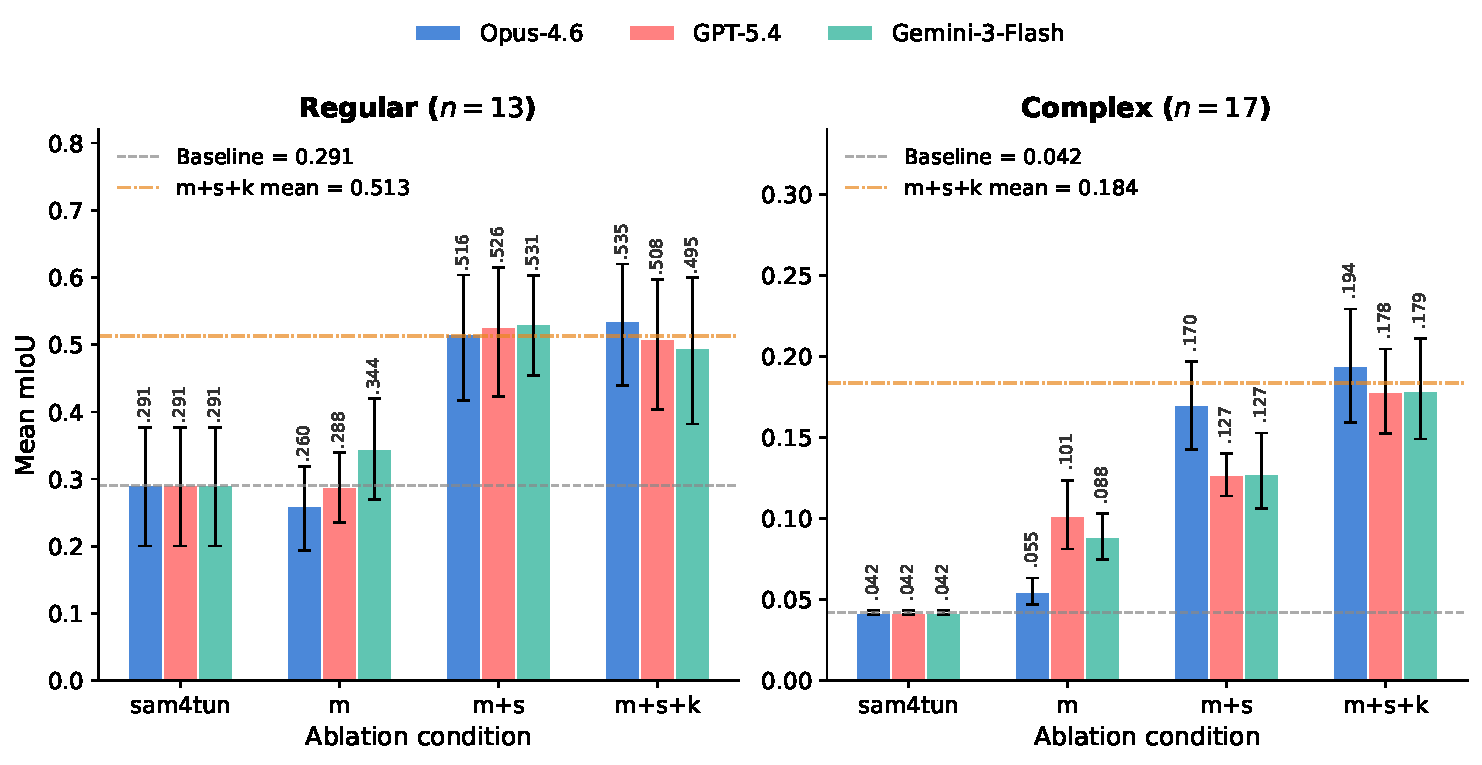
\includegraphics[width=\textwidth]{figs/ablation_bar.pdf}
\caption{Step-wise ablation results split by tunnel family. The baseline (dashed lines) shows the starting point for each family. State produces the dominant jump in both families. Knowledge adds a smaller increment, most pronounced on complex tunnels. Error bars represent bootstrap 95\% CIs.}
\label{fig:ablation-bar}
\end{figure*}

\subsection{Ablation analysis}\label{sec:ablation}

To isolate each context component's contribution, Table~\ref{tab:incremental_miou} reports incremental mIoU gains at each ablation step. Fig.~\ref{fig:ablation-bar} visualises the step-wise progression for regular and complex families across all three LLMs.

\begin{table}[ht]
\caption{Incremental mIoU contribution (mean $\Delta$ vs previous level).}\label{tab:incremental_miou}
\begin{tabular*}{\tblwidth}{@{} l c c c @{}}
\toprule
Transition & Opus~4.6 & GPT-5.4 & Gemini~3~Flash \\
\midrule
Baseline $\rightarrow$ m & $-0.006$ & $+0.032$ & $+0.049$ \\
m $\rightarrow$ m+s & $+0.168$ & $+0.117$ & $+0.103$ \\
\textbf{m+s $\rightarrow$ m+s+k} & $\mathbf{+0.016}$ & $\mathbf{+0.022}$ & $\mathbf{+0.011}$ \\
\bottomrule
\end{tabular*}
\end{table}

\textbf{Memory alone} provides an initial anchor but is insufficient and can be harmful. On regular alternated tunnels, memory alone degrades mIoU by $-0.035$ to $-0.055$. Without intermediate feedback, the agent attempts to adapt parameters but cannot verify whether adjustments improve or degrade the pipeline outputs.

\textbf{State is the dominant driver.} Adding state produces the largest incremental gain across all three LLMs (all $p < 0.0001$; paired Cohen's $d = 1.32$--$1.61$, ``very large'' effect). State provides the agent with explicit quantitative evidence of how each stage has transformed the data---radial percentiles for mask bounds, retention rates for denoising aggressiveness, coverage uniformity for upsampling targets. Without state, the agent has only pre-pipeline statistics that may not reflect conditions after unfolding, denoising, or enhancing.

The gain from state specifically requires LLM reasoning: the state characteristics are raw numbers (percentiles, counts, ratios) that must be interpreted in the context of the pipeline's parameter semantics and mapped to appropriate parameter values. A deterministic lookup table could not perform this mapping because (a)~the characteristics are continuous and multidimensional, (b)~the parameter interactions are non-trivial, and (c)~the same characteristic value can warrant different parameter changes depending on the tunnel family.

\textbf{Knowledge adds targeted improvement.} Mean increment $+0.011$ to $+0.022$ (Cohen's $d = 0.11$--$0.31$, ``small''). Bootstrap CIs on the mean increment straddle zero for all three LLMs. However, 21/30 tunnels show positive increments for Opus~4.6 and GPT-5.4 (one-sided binomial $p = 0.021$), and on complex tunnels 15/17 are positive for GPT ($p = 0.001$). Knowledge is most valuable where it supplies tunnel-family-specific configuration that neither memory nor state can provide (e.g., \texttt{ring\_spacing\_constant}\,=\,1.8 vs 1.2, 7~segments per ring, 7.5/5.5 scaling).

\subsection{Cross-model consistency}\label{sec:consistency}

To assess whether the adaptation is model-dependent or driven by objective tunnel conditions, Table~\ref{tab:cross-model} compares the three LLMs on the full m+s+k condition. All three 95\% CIs overlap substantially, confirming that the improvement is driven by the context design rather than a specific LLM architecture or training corpus.

\begin{table}[ht]
\caption{Cross-model summary (m+s+k vs baseline, overall).}\label{tab:cross-model}
\begin{tabular*}{\tblwidth}{@{} l c c c @{}}
\toprule
LLM & Mean $\Delta$mIoU & 95\% CI & Cohen's $d$ \\
\midrule
Opus~4.6 & $+0.178$ & $[0.139,\; 0.216]$ & 1.61 \\
GPT-5.4 & $+0.171$ & $[0.140,\; 0.203]$ & 1.94 \\
Gemini~3~Flash & $+0.163$ & $[0.122,\; 0.203]$ & 1.44 \\
\bottomrule
\end{tabular*}
\end{table}

\subsection{Parameter sensitivity}\label{sec:sensitivity}


Analysis of 270 adapted parameter runs  (30 tunnels × 3 LLMs × 3 context settings) identified 18 parameters that all three LLMs consistently adjust (Tables~\ref{tab:critical-params}. Of these, 11 are tunnel-responsive ($\text{CV} \geq 0.06$): their adapted values vary systematically with tunnel geometry, clustering by tunnel family. The remaining 7 parameters behave as baseline corrections ($\text{CV} \approx 0$), taking the same improved value on every tunnel regardless of geometry, indicating approximately seven suboptimal SAM4Tun defaults that all three LLMs independently correct to the same values.

\begin{table*}[t]
\caption{Critical parameters identified across all three LLMs (18 total). \emph{Tunnel-responsive} parameters ($\text{CV} \geq 0.06$) vary with tunnel geometry; \emph{baseline corrections} ($\text{CV} \approx 0$) converge to a fixed improved value.}\label{tab:critical-params}
\begin{tabular*}{\textwidth}{@{\extracolsep{\fill}} l l l c c l @{}}
\toprule
Stage & Parameter & Behaviour & Tunnels & CV & Adapted range / correction \\
\midrule
Unfolding & \texttt{diameter} & Responsive & 27/30 & 0.072 & [5.31, 7.6] \\
\midrule
Denoising & \texttt{mask\_r\_low} & Responsive & 30/30 & 0.082 & [2.09, 3.75] \\
Denoising & \texttt{mask\_r\_high} & Responsive & 30/30 & 0.147 & [2.78, 4.38] \\
Denoising & \texttt{default\_cutoff\_z} & Responsive & 29/30 & 0.142 & [2.65, 6.27] \\
Denoising & \texttt{z\_step} & Responsive & 30/30 & 0.181 & [0.003, 0.005] \\
Denoising & \texttt{smooth\_win} & Correction & 30/30 & $\approx$0 & 3 $\rightarrow$ 5 \\
Denoising & \texttt{smooth\_offset} & Correction & 30/30 & $\approx$0 & $-$0.003 $\rightarrow$ $-$0.002 \\
Denoising & \texttt{grad\_thresh} & Correction & 30/30 & $\approx$0 & 0.2 $\rightarrow$ 0.15 \\
Denoising & \texttt{y\_step} & Correction & 30/30 & $\approx$0 & 0.5 $\rightarrow$ 0.4 \\
\midrule
Enhancing & \texttt{inter\_radius} & Responsive & 30/30 & 0.130 & [0.03, 0.08] \\
Enhancing & \texttt{upsampling\_stage1} & Responsive & 30/30 & 0.064 & [0.055, 0.11] \\
Enhancing & \texttt{curv\_thresh} & Correction & 30/30 & $\approx$0 & 0.0005 $\rightarrow$ 0.005 \\
Enhancing & \texttt{depth\_low} & Correction & 30/30 & $\approx$0 & 0.003 $\rightarrow$ 0.005 \\
Enhancing & \texttt{depth\_high} & Correction & 30/30 & $\approx$0 & 0.008 $\rightarrow$ 0.015 \\
\midrule
Prompting & \texttt{hough\_thresh\_obliq} & Responsive & 30/30 & 0.188 & [20, 83] \\
Prompting & \texttt{hough\_thresh\_horiz} & Responsive & 30/30 & 0.204 & [20, 83] \\
Prompting & \texttt{hough\_thresh\_vert} & Responsive & 28/30 & 0.219 & [320, 980] \\
Prompting & \texttt{processing.padding} & Responsive & 29/30 & 0.265 & [160, 419] \\
\bottomrule
\end{tabular*}
\end{table*}



% ══════════════════════════════════════════════════════════════════════════
\section{Discussion}\label{sec:discussion}
% ══════════════════════════════════════════════════════════════════════════

\subsection{Key findings}

The results support the claim that LLM-driven parameter adaptation improves segmentation adaptability across varying tunnel conditions. The adapted pipeline achieves significantly higher mean mIoU than the fixed baseline across tunnel families that differ from the reference, consistently across three independent LLMs. Three findings are central. First, \textbf{state is the dominant driver} ($+0.103$ to $+0.168$ mIoU), because it provides explicit quantitative evidence of how each pipeline stage has transformed the data. Second, \textbf{memory alone is insufficient}: without intermediate feedback, agents make premature adjustments. Third, \textbf{knowledge provides targeted rather than uniform improvement}, most valuable for complex tunnels requiring family-specific configuration.

\subsection{Role of LLM reasoning}

The improvement is specifically attributable to LLM-based reasoning for three reasons. First, the baseline already executes the expert's deterministic rules, and it fails on tunnels outside its design envelope. Second, the state characteristics are raw numeric summaries that require interpretive reasoning to map to parameter values; no deterministic lookup table is provided. Third, three independent LLMs from different providers produce convergent adaptations, ruling out model-specific artefacts and confirming that the reasoning process, interpreting characteristics in the context of parameter semantics, is the source of improvement.


\subsection{Practical implications}

From a deployment perspective, a domain expert calibrates the pipeline on a single reference tunnel, encodes the resulting knowledge into structured documents, and deploys R4Tun to adapt parameters for previously unseen tunnels. This workflow carries four practical advantages: (i)~manual retuning effort is substantially reduced, as the agent autonomously generates tunnel-specific configurations; (ii)~chain-of-thought reasoning traces accompany every adapted parameter set, enabling engineers to audit each adjustment; (iii)~performance degrades gracefully, remaining at or near the baseline rather than collapsing when adaptation offers no benefit; and (iv)~no model retraining or labelled target-domain data is required.

\subsection{Limitations}\label{sec:limitations}

R4Tun was evaluated exclusively on the SAM4Tun pipeline and the Seg2Tunnel dataset; as a result, its transferability to other point-cloud processing pipelines and datasets requires further testing. All adaptation is anchored to a single expert-tuned reference parameter set, which offers little help for complex tunnels, where absolute mIoU remains between 0.169 and 0.177. Alternative approaches such as Bayesian optimisation may narrow this gap further. The interpretability of the generated reasoning traces has not been validated through a formal user study with practising engineers. Finally, parameters are adapted in a single forward pass without iterative self-correction, leaving potential gains from closed-loop refinement unexplored.


% ══════════════════════════════════════════════════════════════════════════
\section{Conclusions}\label{sec:conclusions}
% ══════════════════════════════════════════════════════════════════════════

Consistent segmentation of segmental tunnel linings from point clouds remains challenging when tunnel conditions diverge from the expert-tuned reference. This paper presented R4Tun, a reasoning-driven multi-agent framework that augments a fixed segmentation pipeline with an LLM-driven adaptation layer. Rather than replacing the underlying geometric operators, R4Tun provides a structured mechanism to compare new tunnels against the baseline configuration, interpret compact geometric and statistical summaries of intermediate pipeline state, and apply bounded, context-aware parameter updates accompanied by logged natural-language reasoning traces. This preserves the reproducibility and determinism of the original pipeline while improving both adaptability and transparency: engineers can inspect why parameters change, constrain that behaviour, and revise the encoded memory and knowledge as their understanding evolves.

Evaluated on 30 subsets spanning 13 regular and 17 complex tunnels with three independent LLMs, the full memory\,+\,state\,+\,knowledge design improved mean mIoU from 0.150 to 0.313--0.328 (bootstrap 95\,\% CIs exclude zero for all three LLMs). The ablation study identified state as the dominant driver of improvement (paired Cohen's $d > 1.3$), with all three LLMs converging on the same critical parameters and tunnel-family adaptation patterns. Per-class IoU analysis confirmed broad gains across all structural classes for regular tunnels and progressive recovery from near-zero baselines for complex tunnels. Confidence in the headline improvement and the dominance of state is high; confidence in the knowledge increment is low-to-moderate; these ratings are detailed in Table~\ref{tab:confidence}.

The key contributions are threefold: (i)~the introduction of R4Tun as a reasoning-driven framework that integrates context-aware parameter adaptation with reflective evaluation for automated tunnel point-cloud segmentation; (ii)~a reasoning-based adaptation mechanism using LLMs that reduces reliance on expert-driven tuning while enhancing transparency in decision-making; and (iii)~demonstration that deterministic, expert-designed inspection pipelines need not be rigid or disposable in the face of data variation---by exposing internal state as structured summaries, constraining parameter updates, and requiring explicit justifications, a multi-agent reasoning layer can turn a fixed pipeline into an adaptive framework without altering its core algorithms.

In line with the limitations discussed in Section~\ref{sec:limitations}, future work could enrich the set of anchoring references by encoding multiple expert-designed configurations for atypical tunnels, extend reflection beyond a single coverage-based signal to multi-stage criteria that jointly consider coverage, class balance, and geometric continuity, and validate R4Tun on broader tunnel typologies and acquisition conditions. For infrastructure engineers, R4Tun suggests a practical middle ground between brittle but interpretable rule-based systems and powerful but opaque learning-based models, in which existing tools are retained while adaptability and transparency are systematically improved.

% ══════════════════════════════════════════════════════════════════════════
% Data availability, declarations, etc.
% ══════════════════════════════════════════════════════════════════════════

\section*{Data availability}

The source code, adapted parameters, and evaluation scripts are available at \url{https://github.com/Tao-Robominds/R4Tun}. The Seg2Tunnel dataset is publicly available.

\section*{Declaration of competing interest}

The authors declare that they have no known competing financial interests or personal relationships that could have appeared to influence the work reported in this paper.

\section*{Declaration of generative AI use}

During the preparation of this work, the authors used large language models (Opus~4.6, GPT-5.4, Gemini~3~Flash) as the core experimental subjects of the study. The LLMs were also used for language editing and organisation of the manuscript. The authors reviewed and edited all content and take full responsibility for the content of the publication.

%\printcredits  % Uncomment if cas-dc supports it in your version

% Appendices in external file
% ══════════════════════════════════════════════════════════════════════════
% Appendices — included via % ══════════════════════════════════════════════════════════════════════════
% Appendices — included via % ══════════════════════════════════════════════════════════════════════════
% Appendices — included via \input{appendices} from main document
% ══════════════════════════════════════════════════════════════════════════

\FloatBarrier
% \clearpage
\appendix

\section{Baseline parameter tables}\label{app:params}
Tables~\ref{tab:unfold-params}--\ref{tab:detect-params} report the SAM4Tun baseline parameter values used as the reference configuration for all adaptation experiments.

\begin{table}[ht]
\caption{Unfolding parameters (sam4tun baseline).}\label{tab:unfold-params}
\begin{tabular*}{\tblwidth}{@{} l c @{}}
\toprule
Parameter & Value \\
\midrule
delta & 0.005 \\
slice\_spacing\_factor & 1.2 \\
vertical\_filter\_window & 4.5 \\
ransac\_threshold & 1 \\
ransac\_probability & 0.9 \\
ransac\_inlier\_ratio & 0.75 \\
ransac\_sample\_size & 5 \\
polynomial\_degree & 3 \\
num\_samples\_factor & 1210 \\
diameter & 5.5 \\
\bottomrule
\end{tabular*}
\end{table}

\begin{table}[ht]
\caption{Denoising parameters (sam4tun baseline).}\label{tab:denoise-params}
\begin{tabular*}{\tblwidth}{@{} l c @{}}
\toprule
Parameter & Value \\
\midrule
mask\_r\_low & 2.7 \\
mask\_r\_high & 2.8 \\
y\_step & 0.5 \\
z\_step & 0.001 \\
grad\_threshold & 0.2 \\
smoothing\_window\_size & 3 \\
smoothing\_offset & $-0.003$ \\
default\_cutoff\_z & 2.7 \\
\bottomrule
\end{tabular*}
\end{table}

\begin{table}[ht]
\caption{Enhancing parameters (sam4tun baseline).}\label{tab:enhance-params}
\begin{tabular*}{\tblwidth}{@{} l c @{}}
\toprule
Parameter & Value \\
\midrule
upsamp\_stage1\_target\_dist & 0.08 \\
upsamp\_stage2\_target\_dist & 0.04 \\
upsamp\_stage3\_target\_dist & 0.02 \\
curvature\_threshold & 0.0005 \\
depth\_threshold\_low & 0.003 \\
depth\_threshold\_high & 0.01 \\
inter\_radius & 0.06 \\
duplicate\_threshold & 0.02 \\
num\_neighbors & 20 \\
num\_interpolations & 2 \\
resolution & 0.005 \\
window\_size & 9 \\
\bottomrule
\end{tabular*}
\end{table}

\begin{table}[ht]
\caption{Detecting parameters (sam4tun baseline).}\label{tab:detect-params}
\begin{tabular*}{\tblwidth}{@{} l c @{}}
\toprule
Parameter & Value \\
\midrule
binary\_threshold & 127 \\
morph\_kernel\_size & [3, 3] \\
dilation\_iterations & 1 \\
hough\_thresh\_oblique & 50 \\
minLineLength\_oblique & 100 \\
maxLineGap\_oblique & 40 \\
hough\_thresh\_horiz & 50 \\
minLineLength\_horiz & 100 \\
maxLineGap\_horiz & 10 \\
hough\_thresh\_vert & 500 \\
angle\_range\_obliq\_pos & [6, 9] \\
angle\_range\_obliq\_neg & [$-9$, $-6$] \\
merge\_distance & 3 \\
ring\_spacing\_constant & 1.2 \\
resolution & 0.005 \\
\bottomrule
\end{tabular*}
\end{table}

\section{Tunnel characteristics}\label{app:chars}
Table~\ref{tab:chars} summarises the characteriser fields used to describe each tunnel and to populate the per-stage state provided to the agents.

\begin{table}[ht]
\caption{Characteriser fields by stage. Raw fields are available to all stages; each subsequent group becomes available after the corresponding stage completes.}\label{tab:chars}
\begin{tabular*}{\columnwidth}{@{\extracolsep{\fill}} l p{0.72\columnwidth} @{}}
\toprule
Source & Fields \\
\midrule
\multirow{3}{*}{Raw} & estimated diameter, tunnel length, tunnel height \\
 & $z$-range (min, max) \\
 & mean / median / min nearest-neighbour distance \\
\midrule
\multirow{4}{*}{Unfolded} & $r$-percentiles ($p_{10}$, $p_{99}$), $h$-span, $\theta$-span, $\theta$-range \\
 & median / std nearest-neighbour distance \\
 & intensity median, intensity min \\
\midrule
\multirow{3}{*}{Denoised} & mean / median / std nearest-neighbour distance \\
 & estimated diameter, tunnel length, surface completeness \\
 & surface regularity, average curvature, section curvatures \\
\midrule
\multirow{3}{*}{Enhanced} & total points, median / mean nearest-neighbour distance \\
 & coverage uniformity \\
 & template spacing suitability, current median spacing \\
% Detected-stage fields are omitted because the segmenting stage does not receive stage-specific state beyond the shared raw/enhanced summaries.
\bottomrule
\end{tabular*}
\end{table}

\section{Worked CoT example}\label{app:cot}

The following is a condensed excerpt from the chain-of-thought trace produced by the denoising agent for a complex tunnel (4-1, diameter 7.5\,m, Opus-4.6, m+s+k condition).

\emph{Step~1---Anchoring.}
Current tunnel diameter is 7.5\,m (reference: 5.5\,m, +36\,\%). Unfolded $r$-percentile $p_{10} = 2.63$, $p_{99} = 4.02$ (reference: $p_{10} = 2.37$, $p_{99} = 2.81$). Point density is 1{,}842\,pts/m$^3$ (reference: 2{,}466\,pts/m$^3$, $-$25\,\%).

\emph{Step~2---Diagnostic inspection.}
Large-diameter, moderate-sparse. T4/T5 complex family.
\emph{mask\_r\_low} and \emph{mask\_r\_high} calibrated for 5.5\,m; must widen. \emph{z\_step} must increase for lower density. \emph{default\_cutoff\_z} must increase to cover radial extent to 4.0+.

\emph{Step~3---Parameter adaptation.}
\emph{mask\_r\_low} $= 2.63$ (aligned with $p_{10}$). \emph{mask\_r\_high} $= 4.05$ (above $p_{99} = 4.02$). \emph{z\_step} $= 0.004$ (scaled by density ratio). \emph{default\_cutoff\_z} $= 4.10$.

\emph{Step~4---Validation.}
\emph{mask\_r\_low} (2.63) $<$ \emph{mask\_r\_high} (4.05). Both within physical radius. \emph{default\_cutoff\_z} (4.10) $>$ \emph{mask\_r\_high}.

\emph{Step~5---JSON output.}
\begin{verbatim}
    {
      "delta": 0.007,
      "slice_spacing_factor": 0.8,
      "vertical_filter_window": 7.5,
      "ransac_threshold": 1.5,
      "ransac_probability": 0.9,
      "ransac_inlier_ratio": 0.75,
      "ransac_sample_size": 6,
      "ransac_initial_iterations": 999,
      "ransac_inlier_threshold_multiplier": 0.8,
      "polynomial_degree": 2,
      "num_samples_factor": 1210,
      "t_extrapolation_start": -20,
      "t_extrapolation_end": 20,
      "diameter": 7.5,
      "batch_size": 1000000,
      "n_jobs": 12
    }
\end{verbatim}

\begin{table}[ht]
\caption{Worked example output (Denoising, Tunnel~4-1).}\label{tab:cot-example}
\begin{tabular*}{\tblwidth}{@{} l c c l @{}}
\toprule
Parameter & Baseline & Adapted & Rationale \\
\midrule
mask\_r\_low & 2.7 & 2.63 & Aligned with $p_{10}$ \\
mask\_r\_high & 2.8 & 4.05 & Above $p_{99}$ \\
z\_step & 0.001 & 0.004 & Density ratio \\
default\_cutoff\_z & 2.7 & 4.10 & Full radial extent \\
smooth\_win & 3 & 5 & Baseline correction \\
\bottomrule
\end{tabular*}
\end{table}

The same parameter keys are adapted by GPT-5.4 and Gemini~3~Flash with values within $\pm 5$\,\% of the Opus outputs for this tunnel.

\section{Context components: denoising agent example}\label{app:context}

Tables~\ref{tab:cot-example} and~\ref{tab:context-example} provide a worked denoising example and the corresponding context components assembled for tunnel~4-1 (m+s+k condition, Opus~4.6).

\begin{table*}[ht]
\caption{Context components for the denoising agent (Tunnel~4-1, m+s+k).}\label{tab:context-example}
\begin{tabular*}{\textwidth}{@{} l l @{}}
\toprule
Component & Content \\
\midrule
\multirow{4}{*}{Memory} & Reference: diameter $= 5.5$\,m, density $= 2{,}466$\,pts/m$^3$, $p_{10} = 2.37$, $p_{99} = 2.81$ \\
 & Target: diameter $= 7.5$\,m, density $= 1{,}842$\,pts/m$^3$, $p_{10} = 2.63$, $p_{99} = 4.02$ \\
 & Baseline: mask\_r\_low $= 2.7$, mask\_r\_high $= 2.8$, \\
 & \hspace{2em} z\_step $= 0.001$, smooth\_win $= 3$ \\
\midrule
\multirow{2}{*}{State} & Unfolded (ref): h\_span $= 13.21$, theta\_span $= 5.78$, nn\_median $= 0.0042$ \\
 & Unfolded (4-1): h\_span $= 6.08$, theta\_span $= 7.65$, nn\_median $= 0.0086$ \\
\midrule
\multirow{3}{*}{Knowledge} & Classification: large-diameter if diameter $> 6.5$\,m; moderate-sparse if density $\in [1500, 2000]$ \\
 & Diagnostic: mask\_r\_low $\approx p_{10}$; mask\_r\_high $> p_{99}$; z\_step scales inversely with density \\
 & Defaults: smooth\_win $= 5$ (proven correction) \\
\bottomrule
\end{tabular*}
\end{table*}

\section{On-site rules baseline specification}\label{app:rules}

The rules baseline uses only field-observable inputs and adjusts five parameters from the sam4tun defaults. All other parameters retain their expert-tuned values.

\begin{table}[ht]
\caption{On-site rules baseline: inputs and rule-driven parameters.}\label{tab:rules-spec}
\begin{tabular*}{\tblwidth}{@{} l l l @{}}
\toprule
Stage & Parameter & Rule \\
\midrule
Unfolding & \texttt{diameter} & $= d_{\mathrm{measured}}$ \\
Denoising & \texttt{mask\_r\_low} & $= d/2 - 0.15$ \\
Denoising & \texttt{mask\_r\_high} & $= d/2 + 0.15$ \\
Denoising & \texttt{default\_cutoff\_z} & $= \texttt{mask\_r\_high} + 0.05$ \\
Segmenting & \texttt{ring\_spacing\_constant} & $= L_{\mathrm{ring}}$ (1.2 or 1.8\,m) \\
Segmenting & \texttt{segment\_per\_ring} & $= 6$ (T1--T3) or $7$ (T4--T5) \\
\bottomrule
\end{tabular*}
\end{table}

\noindent Inputs per tunnel: nominal diameter $d$ (design drawings), tunnel family (visual inspection), ring length $L_{\mathrm{ring}}$ (drawings), and segment count (counted visually). For T4--T5 tunnels, SAM template dimensions (\texttt{segment\_width}, \texttt{K\_height}, \texttt{AB\_height}) are scaled by $d/5.5$ and $L_\mathrm{ring}/1.2$ from the 5.5\,m reference. No characteriser output, pipeline intermediate state, or domain-knowledge document is used.

\section{Performance distribution}\label{app:distribution}
Table~\ref{tab:distribution} summarises the distribution of mIoU across tunnels (reported as the mean across the three LLMs for each condition).

\begin{table}[ht]
\caption{Performance distribution (mean across 3 LLMs).}\label{tab:distribution}
\begin{tabular*}{\tblwidth}{@{} l c c c c c @{}}
\toprule
Metric & sam4tun & rules & memory & m+s & m+s+k \\
\midrule
Mean mIoU & 0.150 & 0.201 & 0.175 & 0.304 & 0.320 \\
Std & 0.166 & 0.132 & 0.136 & 0.228 & 0.218 \\
Min & 0.032 & 0.000 & 0.042 & 0.082 & 0.072 \\
Max & 0.532 & 0.484 & 0.471 & 0.682 & 0.679 \\
\bottomrule
\end{tabular*}
\end{table}

\section{Per-class IoU breakdown}\label{app:perclass}

Tables~\ref{tab:perclass-regular} and~\ref{tab:perclass-complex} report per-class IoU for Opus~4.6 (representative; other LLMs show the same pattern) alongside the rules baseline. For regular tunnels, rules achieve per-class IoU comparable to sam4tun while all LLM conditions improve roughly uniformly. For complex tunnels (rules $n=17$ including 3 failed tunnels scored as zero), rules recover segment structure from near-zero for most classes but not K-block; the LLM conditions achieve further improvement on regular tunnels. B2-block remains the hardest class, requiring the 7-segment layout guidance from the knowledge component.

\begin{table}[ht]
\caption{Per-class IoU---Regular tunnels ($n=13$, 6-class, Opus~4.6).}\label{tab:perclass-regular}
\begin{tabular*}{\tblwidth}{@{} l c c c c c @{}}
\toprule
Class & sam4tun & rules & memory & m+s & m+s+k \\
\midrule
Background & 0.640 & 0.597 & 0.559 & 0.741 & 0.751 \\
K-block & 0.192 & 0.222 & 0.129 & 0.373 & 0.386 \\
B1-block & 0.261 & 0.250 & 0.206 & 0.527 & 0.540 \\
A1-block & 0.253 & 0.263 & 0.276 & 0.537 & 0.542 \\
A2-block & 0.150 & 0.144 & 0.159 & 0.380 & 0.420 \\
A3-block & 0.286 & 0.289 & 0.259 & 0.519 & 0.550 \\
B2-block & 0.256 & 0.236 & 0.232 & 0.534 & 0.558 \\
\bottomrule
\end{tabular*}
\end{table}

\begin{table}[ht]
\caption{Per-class IoU---Complex tunnels ($n=17$, 7-class, Opus~4.6). Rules include 3 failed tunnels scored as zero.}\label{tab:perclass-complex}
\begin{tabular*}{\tblwidth}{@{} l c c c c c @{}}
\toprule
Class & sam4tun & rules & memory & m+s & m+s+k \\
\midrule
Background & 0.337 & 0.534 & 0.358 & 0.513 & 0.520 \\
K-block & 0.000 & 0.000 & 0.034 & 0.183 & 0.159 \\
B1-block & 0.000 & 0.041 & 0.001 & 0.084 & 0.135 \\
A1-block & 0.000 & 0.072 & 0.005 & 0.128 & 0.155 \\
A2-block & 0.000 & 0.083 & 0.006 & 0.143 & 0.116 \\
A3-block & 0.000 & 0.149 & 0.017 & 0.092 & 0.119 \\
A4-block & 0.000 & 0.116 & 0.019 & 0.100 & 0.104 \\
B2-block & 0.000 & 0.099 & 0.000 & 0.000 & 0.043 \\
\bottomrule
\end{tabular*}
\end{table}

\section{Runtime and API calls}\label{app:practical}
Table~\ref{tab:practical} reports runtime and API-call counts for the experimental setup.

\begin{table}[ht]
\caption{Runtime and API calls.}\label{tab:practical}
\begin{tabular*}{\tblwidth}{@{} l l @{}}
\toprule
Metric & Value \\
\midrule
LLM API calls per tunnel & 4 (one per stage) \\
Total API calls (full ablation) & 150 per condition per LLM \\
Wall-clock time per tunnel & $\sim$24\,min \\
GPU & Single NVIDIA RTX~5060 \\
Retraining required & None \\
Labelled data required & None (GT for evaluation only) \\
\bottomrule
\end{tabular*}
\end{table}
 from main document
% ══════════════════════════════════════════════════════════════════════════

\FloatBarrier
% \clearpage
\appendix

\section{Baseline parameter tables}\label{app:params}
Tables~\ref{tab:unfold-params}--\ref{tab:detect-params} report the SAM4Tun baseline parameter values used as the reference configuration for all adaptation experiments.

\begin{table}[ht]
\caption{Unfolding parameters (sam4tun baseline).}\label{tab:unfold-params}
\begin{tabular*}{\tblwidth}{@{} l c @{}}
\toprule
Parameter & Value \\
\midrule
delta & 0.005 \\
slice\_spacing\_factor & 1.2 \\
vertical\_filter\_window & 4.5 \\
ransac\_threshold & 1 \\
ransac\_probability & 0.9 \\
ransac\_inlier\_ratio & 0.75 \\
ransac\_sample\_size & 5 \\
polynomial\_degree & 3 \\
num\_samples\_factor & 1210 \\
diameter & 5.5 \\
\bottomrule
\end{tabular*}
\end{table}

\begin{table}[ht]
\caption{Denoising parameters (sam4tun baseline).}\label{tab:denoise-params}
\begin{tabular*}{\tblwidth}{@{} l c @{}}
\toprule
Parameter & Value \\
\midrule
mask\_r\_low & 2.7 \\
mask\_r\_high & 2.8 \\
y\_step & 0.5 \\
z\_step & 0.001 \\
grad\_threshold & 0.2 \\
smoothing\_window\_size & 3 \\
smoothing\_offset & $-0.003$ \\
default\_cutoff\_z & 2.7 \\
\bottomrule
\end{tabular*}
\end{table}

\begin{table}[ht]
\caption{Enhancing parameters (sam4tun baseline).}\label{tab:enhance-params}
\begin{tabular*}{\tblwidth}{@{} l c @{}}
\toprule
Parameter & Value \\
\midrule
upsamp\_stage1\_target\_dist & 0.08 \\
upsamp\_stage2\_target\_dist & 0.04 \\
upsamp\_stage3\_target\_dist & 0.02 \\
curvature\_threshold & 0.0005 \\
depth\_threshold\_low & 0.003 \\
depth\_threshold\_high & 0.01 \\
inter\_radius & 0.06 \\
duplicate\_threshold & 0.02 \\
num\_neighbors & 20 \\
num\_interpolations & 2 \\
resolution & 0.005 \\
window\_size & 9 \\
\bottomrule
\end{tabular*}
\end{table}

\begin{table}[ht]
\caption{Detecting parameters (sam4tun baseline).}\label{tab:detect-params}
\begin{tabular*}{\tblwidth}{@{} l c @{}}
\toprule
Parameter & Value \\
\midrule
binary\_threshold & 127 \\
morph\_kernel\_size & [3, 3] \\
dilation\_iterations & 1 \\
hough\_thresh\_oblique & 50 \\
minLineLength\_oblique & 100 \\
maxLineGap\_oblique & 40 \\
hough\_thresh\_horiz & 50 \\
minLineLength\_horiz & 100 \\
maxLineGap\_horiz & 10 \\
hough\_thresh\_vert & 500 \\
angle\_range\_obliq\_pos & [6, 9] \\
angle\_range\_obliq\_neg & [$-9$, $-6$] \\
merge\_distance & 3 \\
ring\_spacing\_constant & 1.2 \\
resolution & 0.005 \\
\bottomrule
\end{tabular*}
\end{table}

\section{Tunnel characteristics}\label{app:chars}
Table~\ref{tab:chars} summarises the characteriser fields used to describe each tunnel and to populate the per-stage state provided to the agents.

\begin{table}[ht]
\caption{Characteriser fields by stage. Raw fields are available to all stages; each subsequent group becomes available after the corresponding stage completes.}\label{tab:chars}
\begin{tabular*}{\columnwidth}{@{\extracolsep{\fill}} l p{0.72\columnwidth} @{}}
\toprule
Source & Fields \\
\midrule
\multirow{3}{*}{Raw} & estimated diameter, tunnel length, tunnel height \\
 & $z$-range (min, max) \\
 & mean / median / min nearest-neighbour distance \\
\midrule
\multirow{4}{*}{Unfolded} & $r$-percentiles ($p_{10}$, $p_{99}$), $h$-span, $\theta$-span, $\theta$-range \\
 & median / std nearest-neighbour distance \\
 & intensity median, intensity min \\
\midrule
\multirow{3}{*}{Denoised} & mean / median / std nearest-neighbour distance \\
 & estimated diameter, tunnel length, surface completeness \\
 & surface regularity, average curvature, section curvatures \\
\midrule
\multirow{3}{*}{Enhanced} & total points, median / mean nearest-neighbour distance \\
 & coverage uniformity \\
 & template spacing suitability, current median spacing \\
% Detected-stage fields are omitted because the segmenting stage does not receive stage-specific state beyond the shared raw/enhanced summaries.
\bottomrule
\end{tabular*}
\end{table}

\section{Worked CoT example}\label{app:cot}

The following is a condensed excerpt from the chain-of-thought trace produced by the denoising agent for a complex tunnel (4-1, diameter 7.5\,m, Opus-4.6, m+s+k condition).

\emph{Step~1---Anchoring.}
Current tunnel diameter is 7.5\,m (reference: 5.5\,m, +36\,\%). Unfolded $r$-percentile $p_{10} = 2.63$, $p_{99} = 4.02$ (reference: $p_{10} = 2.37$, $p_{99} = 2.81$). Point density is 1{,}842\,pts/m$^3$ (reference: 2{,}466\,pts/m$^3$, $-$25\,\%).

\emph{Step~2---Diagnostic inspection.}
Large-diameter, moderate-sparse. T4/T5 complex family.
\emph{mask\_r\_low} and \emph{mask\_r\_high} calibrated for 5.5\,m; must widen. \emph{z\_step} must increase for lower density. \emph{default\_cutoff\_z} must increase to cover radial extent to 4.0+.

\emph{Step~3---Parameter adaptation.}
\emph{mask\_r\_low} $= 2.63$ (aligned with $p_{10}$). \emph{mask\_r\_high} $= 4.05$ (above $p_{99} = 4.02$). \emph{z\_step} $= 0.004$ (scaled by density ratio). \emph{default\_cutoff\_z} $= 4.10$.

\emph{Step~4---Validation.}
\emph{mask\_r\_low} (2.63) $<$ \emph{mask\_r\_high} (4.05). Both within physical radius. \emph{default\_cutoff\_z} (4.10) $>$ \emph{mask\_r\_high}.

\emph{Step~5---JSON output.}
\begin{verbatim}
    {
      "delta": 0.007,
      "slice_spacing_factor": 0.8,
      "vertical_filter_window": 7.5,
      "ransac_threshold": 1.5,
      "ransac_probability": 0.9,
      "ransac_inlier_ratio": 0.75,
      "ransac_sample_size": 6,
      "ransac_initial_iterations": 999,
      "ransac_inlier_threshold_multiplier": 0.8,
      "polynomial_degree": 2,
      "num_samples_factor": 1210,
      "t_extrapolation_start": -20,
      "t_extrapolation_end": 20,
      "diameter": 7.5,
      "batch_size": 1000000,
      "n_jobs": 12
    }
\end{verbatim}

\begin{table}[ht]
\caption{Worked example output (Denoising, Tunnel~4-1).}\label{tab:cot-example}
\begin{tabular*}{\tblwidth}{@{} l c c l @{}}
\toprule
Parameter & Baseline & Adapted & Rationale \\
\midrule
mask\_r\_low & 2.7 & 2.63 & Aligned with $p_{10}$ \\
mask\_r\_high & 2.8 & 4.05 & Above $p_{99}$ \\
z\_step & 0.001 & 0.004 & Density ratio \\
default\_cutoff\_z & 2.7 & 4.10 & Full radial extent \\
smooth\_win & 3 & 5 & Baseline correction \\
\bottomrule
\end{tabular*}
\end{table}

The same parameter keys are adapted by GPT-5.4 and Gemini~3~Flash with values within $\pm 5$\,\% of the Opus outputs for this tunnel.

\section{Context components: denoising agent example}\label{app:context}

Tables~\ref{tab:cot-example} and~\ref{tab:context-example} provide a worked denoising example and the corresponding context components assembled for tunnel~4-1 (m+s+k condition, Opus~4.6).

\begin{table*}[ht]
\caption{Context components for the denoising agent (Tunnel~4-1, m+s+k).}\label{tab:context-example}
\begin{tabular*}{\textwidth}{@{} l l @{}}
\toprule
Component & Content \\
\midrule
\multirow{4}{*}{Memory} & Reference: diameter $= 5.5$\,m, density $= 2{,}466$\,pts/m$^3$, $p_{10} = 2.37$, $p_{99} = 2.81$ \\
 & Target: diameter $= 7.5$\,m, density $= 1{,}842$\,pts/m$^3$, $p_{10} = 2.63$, $p_{99} = 4.02$ \\
 & Baseline: mask\_r\_low $= 2.7$, mask\_r\_high $= 2.8$, \\
 & \hspace{2em} z\_step $= 0.001$, smooth\_win $= 3$ \\
\midrule
\multirow{2}{*}{State} & Unfolded (ref): h\_span $= 13.21$, theta\_span $= 5.78$, nn\_median $= 0.0042$ \\
 & Unfolded (4-1): h\_span $= 6.08$, theta\_span $= 7.65$, nn\_median $= 0.0086$ \\
\midrule
\multirow{3}{*}{Knowledge} & Classification: large-diameter if diameter $> 6.5$\,m; moderate-sparse if density $\in [1500, 2000]$ \\
 & Diagnostic: mask\_r\_low $\approx p_{10}$; mask\_r\_high $> p_{99}$; z\_step scales inversely with density \\
 & Defaults: smooth\_win $= 5$ (proven correction) \\
\bottomrule
\end{tabular*}
\end{table*}

\section{On-site rules baseline specification}\label{app:rules}

The rules baseline uses only field-observable inputs and adjusts five parameters from the sam4tun defaults. All other parameters retain their expert-tuned values.

\begin{table}[ht]
\caption{On-site rules baseline: inputs and rule-driven parameters.}\label{tab:rules-spec}
\begin{tabular*}{\tblwidth}{@{} l l l @{}}
\toprule
Stage & Parameter & Rule \\
\midrule
Unfolding & \texttt{diameter} & $= d_{\mathrm{measured}}$ \\
Denoising & \texttt{mask\_r\_low} & $= d/2 - 0.15$ \\
Denoising & \texttt{mask\_r\_high} & $= d/2 + 0.15$ \\
Denoising & \texttt{default\_cutoff\_z} & $= \texttt{mask\_r\_high} + 0.05$ \\
Segmenting & \texttt{ring\_spacing\_constant} & $= L_{\mathrm{ring}}$ (1.2 or 1.8\,m) \\
Segmenting & \texttt{segment\_per\_ring} & $= 6$ (T1--T3) or $7$ (T4--T5) \\
\bottomrule
\end{tabular*}
\end{table}

\noindent Inputs per tunnel: nominal diameter $d$ (design drawings), tunnel family (visual inspection), ring length $L_{\mathrm{ring}}$ (drawings), and segment count (counted visually). For T4--T5 tunnels, SAM template dimensions (\texttt{segment\_width}, \texttt{K\_height}, \texttt{AB\_height}) are scaled by $d/5.5$ and $L_\mathrm{ring}/1.2$ from the 5.5\,m reference. No characteriser output, pipeline intermediate state, or domain-knowledge document is used.

\section{Performance distribution}\label{app:distribution}
Table~\ref{tab:distribution} summarises the distribution of mIoU across tunnels (reported as the mean across the three LLMs for each condition).

\begin{table}[ht]
\caption{Performance distribution (mean across 3 LLMs).}\label{tab:distribution}
\begin{tabular*}{\tblwidth}{@{} l c c c c c @{}}
\toprule
Metric & sam4tun & rules & memory & m+s & m+s+k \\
\midrule
Mean mIoU & 0.150 & 0.201 & 0.175 & 0.304 & 0.320 \\
Std & 0.166 & 0.132 & 0.136 & 0.228 & 0.218 \\
Min & 0.032 & 0.000 & 0.042 & 0.082 & 0.072 \\
Max & 0.532 & 0.484 & 0.471 & 0.682 & 0.679 \\
\bottomrule
\end{tabular*}
\end{table}

\section{Per-class IoU breakdown}\label{app:perclass}

Tables~\ref{tab:perclass-regular} and~\ref{tab:perclass-complex} report per-class IoU for Opus~4.6 (representative; other LLMs show the same pattern) alongside the rules baseline. For regular tunnels, rules achieve per-class IoU comparable to sam4tun while all LLM conditions improve roughly uniformly. For complex tunnels (rules $n=17$ including 3 failed tunnels scored as zero), rules recover segment structure from near-zero for most classes but not K-block; the LLM conditions achieve further improvement on regular tunnels. B2-block remains the hardest class, requiring the 7-segment layout guidance from the knowledge component.

\begin{table}[ht]
\caption{Per-class IoU---Regular tunnels ($n=13$, 6-class, Opus~4.6).}\label{tab:perclass-regular}
\begin{tabular*}{\tblwidth}{@{} l c c c c c @{}}
\toprule
Class & sam4tun & rules & memory & m+s & m+s+k \\
\midrule
Background & 0.640 & 0.597 & 0.559 & 0.741 & 0.751 \\
K-block & 0.192 & 0.222 & 0.129 & 0.373 & 0.386 \\
B1-block & 0.261 & 0.250 & 0.206 & 0.527 & 0.540 \\
A1-block & 0.253 & 0.263 & 0.276 & 0.537 & 0.542 \\
A2-block & 0.150 & 0.144 & 0.159 & 0.380 & 0.420 \\
A3-block & 0.286 & 0.289 & 0.259 & 0.519 & 0.550 \\
B2-block & 0.256 & 0.236 & 0.232 & 0.534 & 0.558 \\
\bottomrule
\end{tabular*}
\end{table}

\begin{table}[ht]
\caption{Per-class IoU---Complex tunnels ($n=17$, 7-class, Opus~4.6). Rules include 3 failed tunnels scored as zero.}\label{tab:perclass-complex}
\begin{tabular*}{\tblwidth}{@{} l c c c c c @{}}
\toprule
Class & sam4tun & rules & memory & m+s & m+s+k \\
\midrule
Background & 0.337 & 0.534 & 0.358 & 0.513 & 0.520 \\
K-block & 0.000 & 0.000 & 0.034 & 0.183 & 0.159 \\
B1-block & 0.000 & 0.041 & 0.001 & 0.084 & 0.135 \\
A1-block & 0.000 & 0.072 & 0.005 & 0.128 & 0.155 \\
A2-block & 0.000 & 0.083 & 0.006 & 0.143 & 0.116 \\
A3-block & 0.000 & 0.149 & 0.017 & 0.092 & 0.119 \\
A4-block & 0.000 & 0.116 & 0.019 & 0.100 & 0.104 \\
B2-block & 0.000 & 0.099 & 0.000 & 0.000 & 0.043 \\
\bottomrule
\end{tabular*}
\end{table}

\section{Runtime and API calls}\label{app:practical}
Table~\ref{tab:practical} reports runtime and API-call counts for the experimental setup.

\begin{table}[ht]
\caption{Runtime and API calls.}\label{tab:practical}
\begin{tabular*}{\tblwidth}{@{} l l @{}}
\toprule
Metric & Value \\
\midrule
LLM API calls per tunnel & 4 (one per stage) \\
Total API calls (full ablation) & 150 per condition per LLM \\
Wall-clock time per tunnel & $\sim$24\,min \\
GPU & Single NVIDIA RTX~5060 \\
Retraining required & None \\
Labelled data required & None (GT for evaluation only) \\
\bottomrule
\end{tabular*}
\end{table}
 from main document
% ══════════════════════════════════════════════════════════════════════════

\FloatBarrier
% \clearpage
\appendix

\section{Baseline parameter tables}\label{app:params}
Tables~\ref{tab:unfold-params}--\ref{tab:detect-params} report the SAM4Tun baseline parameter values used as the reference configuration for all adaptation experiments.

\begin{table}[ht]
\caption{Unfolding parameters (sam4tun baseline).}\label{tab:unfold-params}
\begin{tabular*}{\tblwidth}{@{} l c @{}}
\toprule
Parameter & Value \\
\midrule
delta & 0.005 \\
slice\_spacing\_factor & 1.2 \\
vertical\_filter\_window & 4.5 \\
ransac\_threshold & 1 \\
ransac\_probability & 0.9 \\
ransac\_inlier\_ratio & 0.75 \\
ransac\_sample\_size & 5 \\
polynomial\_degree & 3 \\
num\_samples\_factor & 1210 \\
diameter & 5.5 \\
\bottomrule
\end{tabular*}
\end{table}

\begin{table}[ht]
\caption{Denoising parameters (sam4tun baseline).}\label{tab:denoise-params}
\begin{tabular*}{\tblwidth}{@{} l c @{}}
\toprule
Parameter & Value \\
\midrule
mask\_r\_low & 2.7 \\
mask\_r\_high & 2.8 \\
y\_step & 0.5 \\
z\_step & 0.001 \\
grad\_threshold & 0.2 \\
smoothing\_window\_size & 3 \\
smoothing\_offset & $-0.003$ \\
default\_cutoff\_z & 2.7 \\
\bottomrule
\end{tabular*}
\end{table}

\begin{table}[ht]
\caption{Enhancing parameters (sam4tun baseline).}\label{tab:enhance-params}
\begin{tabular*}{\tblwidth}{@{} l c @{}}
\toprule
Parameter & Value \\
\midrule
upsamp\_stage1\_target\_dist & 0.08 \\
upsamp\_stage2\_target\_dist & 0.04 \\
upsamp\_stage3\_target\_dist & 0.02 \\
curvature\_threshold & 0.0005 \\
depth\_threshold\_low & 0.003 \\
depth\_threshold\_high & 0.01 \\
inter\_radius & 0.06 \\
duplicate\_threshold & 0.02 \\
num\_neighbors & 20 \\
num\_interpolations & 2 \\
resolution & 0.005 \\
window\_size & 9 \\
\bottomrule
\end{tabular*}
\end{table}

\begin{table}[ht]
\caption{Detecting parameters (sam4tun baseline).}\label{tab:detect-params}
\begin{tabular*}{\tblwidth}{@{} l c @{}}
\toprule
Parameter & Value \\
\midrule
binary\_threshold & 127 \\
morph\_kernel\_size & [3, 3] \\
dilation\_iterations & 1 \\
hough\_thresh\_oblique & 50 \\
minLineLength\_oblique & 100 \\
maxLineGap\_oblique & 40 \\
hough\_thresh\_horiz & 50 \\
minLineLength\_horiz & 100 \\
maxLineGap\_horiz & 10 \\
hough\_thresh\_vert & 500 \\
angle\_range\_obliq\_pos & [6, 9] \\
angle\_range\_obliq\_neg & [$-9$, $-6$] \\
merge\_distance & 3 \\
ring\_spacing\_constant & 1.2 \\
resolution & 0.005 \\
\bottomrule
\end{tabular*}
\end{table}

\section{Tunnel characteristics}\label{app:chars}
Table~\ref{tab:chars} summarises the characteriser fields used to describe each tunnel and to populate the per-stage state provided to the agents.

\begin{table}[ht]
\caption{Characteriser fields by stage. Raw fields are available to all stages; each subsequent group becomes available after the corresponding stage completes.}\label{tab:chars}
\begin{tabular*}{\columnwidth}{@{\extracolsep{\fill}} l p{0.72\columnwidth} @{}}
\toprule
Source & Fields \\
\midrule
\multirow{3}{*}{Raw} & estimated diameter, tunnel length, tunnel height \\
 & $z$-range (min, max) \\
 & mean / median / min nearest-neighbour distance \\
\midrule
\multirow{4}{*}{Unfolded} & $r$-percentiles ($p_{10}$, $p_{99}$), $h$-span, $\theta$-span, $\theta$-range \\
 & median / std nearest-neighbour distance \\
 & intensity median, intensity min \\
\midrule
\multirow{3}{*}{Denoised} & mean / median / std nearest-neighbour distance \\
 & estimated diameter, tunnel length, surface completeness \\
 & surface regularity, average curvature, section curvatures \\
\midrule
\multirow{3}{*}{Enhanced} & total points, median / mean nearest-neighbour distance \\
 & coverage uniformity \\
 & template spacing suitability, current median spacing \\
% Detected-stage fields are omitted because the segmenting stage does not receive stage-specific state beyond the shared raw/enhanced summaries.
\bottomrule
\end{tabular*}
\end{table}

\section{Worked CoT example}\label{app:cot}

The following is a condensed excerpt from the chain-of-thought trace produced by the denoising agent for a complex tunnel (4-1, diameter 7.5\,m, Opus-4.6, m+s+k condition).

\emph{Step~1---Anchoring.}
Current tunnel diameter is 7.5\,m (reference: 5.5\,m, +36\,\%). Unfolded $r$-percentile $p_{10} = 2.63$, $p_{99} = 4.02$ (reference: $p_{10} = 2.37$, $p_{99} = 2.81$). Point density is 1{,}842\,pts/m$^3$ (reference: 2{,}466\,pts/m$^3$, $-$25\,\%).

\emph{Step~2---Diagnostic inspection.}
Large-diameter, moderate-sparse. T4/T5 complex family.
\emph{mask\_r\_low} and \emph{mask\_r\_high} calibrated for 5.5\,m; must widen. \emph{z\_step} must increase for lower density. \emph{default\_cutoff\_z} must increase to cover radial extent to 4.0+.

\emph{Step~3---Parameter adaptation.}
\emph{mask\_r\_low} $= 2.63$ (aligned with $p_{10}$). \emph{mask\_r\_high} $= 4.05$ (above $p_{99} = 4.02$). \emph{z\_step} $= 0.004$ (scaled by density ratio). \emph{default\_cutoff\_z} $= 4.10$.

\emph{Step~4---Validation.}
\emph{mask\_r\_low} (2.63) $<$ \emph{mask\_r\_high} (4.05). Both within physical radius. \emph{default\_cutoff\_z} (4.10) $>$ \emph{mask\_r\_high}.

\emph{Step~5---JSON output.}
\begin{verbatim}
    {
      "delta": 0.007,
      "slice_spacing_factor": 0.8,
      "vertical_filter_window": 7.5,
      "ransac_threshold": 1.5,
      "ransac_probability": 0.9,
      "ransac_inlier_ratio": 0.75,
      "ransac_sample_size": 6,
      "ransac_initial_iterations": 999,
      "ransac_inlier_threshold_multiplier": 0.8,
      "polynomial_degree": 2,
      "num_samples_factor": 1210,
      "t_extrapolation_start": -20,
      "t_extrapolation_end": 20,
      "diameter": 7.5,
      "batch_size": 1000000,
      "n_jobs": 12
    }
\end{verbatim}

\begin{table}[ht]
\caption{Worked example output (Denoising, Tunnel~4-1).}\label{tab:cot-example}
\begin{tabular*}{\tblwidth}{@{} l c c l @{}}
\toprule
Parameter & Baseline & Adapted & Rationale \\
\midrule
mask\_r\_low & 2.7 & 2.63 & Aligned with $p_{10}$ \\
mask\_r\_high & 2.8 & 4.05 & Above $p_{99}$ \\
z\_step & 0.001 & 0.004 & Density ratio \\
default\_cutoff\_z & 2.7 & 4.10 & Full radial extent \\
smooth\_win & 3 & 5 & Baseline correction \\
\bottomrule
\end{tabular*}
\end{table}

The same parameter keys are adapted by GPT-5.4 and Gemini~3~Flash with values within $\pm 5$\,\% of the Opus outputs for this tunnel.

\section{Context components: denoising agent example}\label{app:context}

Tables~\ref{tab:cot-example} and~\ref{tab:context-example} provide a worked denoising example and the corresponding context components assembled for tunnel~4-1 (m+s+k condition, Opus~4.6).

\begin{table*}[ht]
\caption{Context components for the denoising agent (Tunnel~4-1, m+s+k).}\label{tab:context-example}
\begin{tabular*}{\textwidth}{@{} l l @{}}
\toprule
Component & Content \\
\midrule
\multirow{4}{*}{Memory} & Reference: diameter $= 5.5$\,m, density $= 2{,}466$\,pts/m$^3$, $p_{10} = 2.37$, $p_{99} = 2.81$ \\
 & Target: diameter $= 7.5$\,m, density $= 1{,}842$\,pts/m$^3$, $p_{10} = 2.63$, $p_{99} = 4.02$ \\
 & Baseline: mask\_r\_low $= 2.7$, mask\_r\_high $= 2.8$, \\
 & \hspace{2em} z\_step $= 0.001$, smooth\_win $= 3$ \\
\midrule
\multirow{2}{*}{State} & Unfolded (ref): h\_span $= 13.21$, theta\_span $= 5.78$, nn\_median $= 0.0042$ \\
 & Unfolded (4-1): h\_span $= 6.08$, theta\_span $= 7.65$, nn\_median $= 0.0086$ \\
\midrule
\multirow{3}{*}{Knowledge} & Classification: large-diameter if diameter $> 6.5$\,m; moderate-sparse if density $\in [1500, 2000]$ \\
 & Diagnostic: mask\_r\_low $\approx p_{10}$; mask\_r\_high $> p_{99}$; z\_step scales inversely with density \\
 & Defaults: smooth\_win $= 5$ (proven correction) \\
\bottomrule
\end{tabular*}
\end{table*}

\section{On-site rules baseline specification}\label{app:rules}

The rules baseline uses only field-observable inputs and adjusts five parameters from the sam4tun defaults. All other parameters retain their expert-tuned values.

\begin{table}[ht]
\caption{On-site rules baseline: inputs and rule-driven parameters.}\label{tab:rules-spec}
\begin{tabular*}{\tblwidth}{@{} l l l @{}}
\toprule
Stage & Parameter & Rule \\
\midrule
Unfolding & \texttt{diameter} & $= d_{\mathrm{measured}}$ \\
Denoising & \texttt{mask\_r\_low} & $= d/2 - 0.15$ \\
Denoising & \texttt{mask\_r\_high} & $= d/2 + 0.15$ \\
Denoising & \texttt{default\_cutoff\_z} & $= \texttt{mask\_r\_high} + 0.05$ \\
Segmenting & \texttt{ring\_spacing\_constant} & $= L_{\mathrm{ring}}$ (1.2 or 1.8\,m) \\
Segmenting & \texttt{segment\_per\_ring} & $= 6$ (T1--T3) or $7$ (T4--T5) \\
\bottomrule
\end{tabular*}
\end{table}

\noindent Inputs per tunnel: nominal diameter $d$ (design drawings), tunnel family (visual inspection), ring length $L_{\mathrm{ring}}$ (drawings), and segment count (counted visually). For T4--T5 tunnels, SAM template dimensions (\texttt{segment\_width}, \texttt{K\_height}, \texttt{AB\_height}) are scaled by $d/5.5$ and $L_\mathrm{ring}/1.2$ from the 5.5\,m reference. No characteriser output, pipeline intermediate state, or domain-knowledge document is used.

\section{Performance distribution}\label{app:distribution}
Table~\ref{tab:distribution} summarises the distribution of mIoU across tunnels (reported as the mean across the three LLMs for each condition).

\begin{table}[ht]
\caption{Performance distribution (mean across 3 LLMs).}\label{tab:distribution}
\begin{tabular*}{\tblwidth}{@{} l c c c c c @{}}
\toprule
Metric & sam4tun & rules & memory & m+s & m+s+k \\
\midrule
Mean mIoU & 0.150 & 0.201 & 0.175 & 0.304 & 0.320 \\
Std & 0.166 & 0.132 & 0.136 & 0.228 & 0.218 \\
Min & 0.032 & 0.000 & 0.042 & 0.082 & 0.072 \\
Max & 0.532 & 0.484 & 0.471 & 0.682 & 0.679 \\
\bottomrule
\end{tabular*}
\end{table}

\section{Per-class IoU breakdown}\label{app:perclass}

Tables~\ref{tab:perclass-regular} and~\ref{tab:perclass-complex} report per-class IoU for Opus~4.6 (representative; other LLMs show the same pattern) alongside the rules baseline. For regular tunnels, rules achieve per-class IoU comparable to sam4tun while all LLM conditions improve roughly uniformly. For complex tunnels (rules $n=17$ including 3 failed tunnels scored as zero), rules recover segment structure from near-zero for most classes but not K-block; the LLM conditions achieve further improvement on regular tunnels. B2-block remains the hardest class, requiring the 7-segment layout guidance from the knowledge component.

\begin{table}[ht]
\caption{Per-class IoU---Regular tunnels ($n=13$, 6-class, Opus~4.6).}\label{tab:perclass-regular}
\begin{tabular*}{\tblwidth}{@{} l c c c c c @{}}
\toprule
Class & sam4tun & rules & memory & m+s & m+s+k \\
\midrule
Background & 0.640 & 0.597 & 0.559 & 0.741 & 0.751 \\
K-block & 0.192 & 0.222 & 0.129 & 0.373 & 0.386 \\
B1-block & 0.261 & 0.250 & 0.206 & 0.527 & 0.540 \\
A1-block & 0.253 & 0.263 & 0.276 & 0.537 & 0.542 \\
A2-block & 0.150 & 0.144 & 0.159 & 0.380 & 0.420 \\
A3-block & 0.286 & 0.289 & 0.259 & 0.519 & 0.550 \\
B2-block & 0.256 & 0.236 & 0.232 & 0.534 & 0.558 \\
\bottomrule
\end{tabular*}
\end{table}

\begin{table}[ht]
\caption{Per-class IoU---Complex tunnels ($n=17$, 7-class, Opus~4.6). Rules include 3 failed tunnels scored as zero.}\label{tab:perclass-complex}
\begin{tabular*}{\tblwidth}{@{} l c c c c c @{}}
\toprule
Class & sam4tun & rules & memory & m+s & m+s+k \\
\midrule
Background & 0.337 & 0.534 & 0.358 & 0.513 & 0.520 \\
K-block & 0.000 & 0.000 & 0.034 & 0.183 & 0.159 \\
B1-block & 0.000 & 0.041 & 0.001 & 0.084 & 0.135 \\
A1-block & 0.000 & 0.072 & 0.005 & 0.128 & 0.155 \\
A2-block & 0.000 & 0.083 & 0.006 & 0.143 & 0.116 \\
A3-block & 0.000 & 0.149 & 0.017 & 0.092 & 0.119 \\
A4-block & 0.000 & 0.116 & 0.019 & 0.100 & 0.104 \\
B2-block & 0.000 & 0.099 & 0.000 & 0.000 & 0.043 \\
\bottomrule
\end{tabular*}
\end{table}

\section{Runtime and API calls}\label{app:practical}
Table~\ref{tab:practical} reports runtime and API-call counts for the experimental setup.

\begin{table}[ht]
\caption{Runtime and API calls.}\label{tab:practical}
\begin{tabular*}{\tblwidth}{@{} l l @{}}
\toprule
Metric & Value \\
\midrule
LLM API calls per tunnel & 4 (one per stage) \\
Total API calls (full ablation) & 150 per condition per LLM \\
Wall-clock time per tunnel & $\sim$24\,min \\
GPU & Single NVIDIA RTX~5060 \\
Retraining required & None \\
Labelled data required & None (GT for evaluation only) \\
\bottomrule
\end{tabular*}
\end{table}



% ══════════════════════════════════════════════════════════════════════════
% Bibliography
% ══════════════════════════════════════════════════════════════════════════

\clearpage % start Biography on a new page
\section*{Biography}
% TODO: add biography text here

% Natbib requires a BibTeX style; without it, citations stay as “?”
\bibliographystyle{model1-num-names}
\bibliography{references}

\end{document}
